%%%%%%%%%%%%%%%%%%%%%%%%%%%%%%%%%%%%%%%%%%%%%%%%%%%%%%%%%%%%
%%% ELIFE ARTICLE TEMPLATE
%%%%%%%%%%%%%%%%%%%%%%%%%%%%%%%%%%%%%%%%%%%%%%%%%%%%%%%%%%%%
%%% PREAMBLE 
\documentclass[9pt,lineno]{elife}
% Use the onehalfspacing option for 1.5 line spacing
% Use the doublespacing option for 2.0 line spacing
% Please note that these options may affect formatting.

\usepackage{lipsum} % Required to insert dummy text
\usepackage[version=4]{mhchem}
\usepackage{siunitx}
\DeclareSIUnit\Molar{M}
\usepackage{indentfirst} %I prefer to have indents following section headings, I find it to be more consistent in style throughout document
\usepackage{natbib}
\usepackage{float}


\newfloat{suppfile}{thp}{lofsupfile}
%\renewcommand{\thesuppfile}{Supplementary file \arabic{suppfile}}
\floatname{suppfile}{Supplementary file}

\renewcommand{\floatpagefraction}{1}

\newcommand{\jdbcomment}[1]{\emph{\color{red} [#1]}}

%%%%%%%%%%%%%%%%%%%%%%%%%%%%%%%%%%%%%%%%%%%%%%%%%%%%%%%%%%%%
%%% ARTICLE SETUP
%%%%%%%%%%%%%%%%%%%%%%%%%%%%%%%%%%%%%%%%%%%%%%%%%%%%%%%%%%%%
\title{Transcriptional dynamics of influenza virus infection in single cells}

\author[1]{Alistair B. Russell}
\author[2]{Cole Trapnell}
\author[1,2*]{Jesse D. Bloom}
\affil[1]{Basic Sciences Division and Computational Biology Program, Fred Hutchinson Cancer Research Center, Seattle, United States}
\affil[2]{Department of Genome Sciences, University of Washington, Seattle, United States}
\corr{jbloom@fredhutch.org}{}

% \presentadd[\authfn{5}]{eLife Sciences editorial Office, eLife Sciences, Cambridge, United Kingdom}

%%%%%%%%%%%%%%%%%%%%%%%%%%%%%%%%%%%%%%%%%%%%%%%%%%%%%%%%%%%%
%%% ARTICLE START
%%%%%%%%%%%%%%%%%%%%%%%%%%%%%%%%%%%%%%%%%%%%%%%%%%%%%%%%%%%%

\begin{document}

\maketitle

\begin{abstract}
Influenza virus infection induces large changes in cellular transcription.
Previously this has mostly been looked at using bulk measurements
Here we examine the process at the level of single cells.
We find extremely wide variation in the extent of viral gene transcription across infected cells.
IFN induction is very rare.
Some cellular pathways may be consistently altered in cells with high burden of viral transcripts.
Overall, highlights remarkable heterogeneity in the outcome of infection.
\end{abstract}


\section{Introduction}

Heterogeneity is important in a lot of cellular processes even when isogenic~\citep{Shalek:2014ey,Shalek:2013ej}.

Population (genetic) heterogeneity is also important. 
Viral quasispecies, cancer single-cell, etc.
Salmonella paper (PhoP).

Literature on viral burst-size heterogeneity.
This goes back to Delbruck, Andino polio paper~\citep{Schulte:2014br}, the MDCK / flu paper.

Discuss segmented nature of influenza.
Maybe in the context of how this could further increase heterogeneity because there is a lot of potential for entire genes to be missing.
Includes Yewdell and Lowen papers.

\section{Results}

\subsection{Strategy to measure mRNA in single virus-infected cells.}
We performed single-cell mRNA sequencing using a droplet-based system that physically isolates individual cells prior to reverse transcription~\citep{zheng2017massively,Macosko:2015ht,Klein:2015ki}.
Each droplet is associated with a unique \emph{cell barcode} that tags all mRNAs from that cell during reverse-transcription.
A random \emph{unique molecular identifier (UMI)} is additionally appended to each mRNA molecule during reverse transcription.
The 3' ends of the mRNAs are sequenced and mapped to the human and influenza virus transcriptomes to determine transcript identities.
This information is combined with that provided by the UMIs and cell barcodes to quantify the number of molecules of each mRNA species that have been captured for each cell.

Infected cells will express viral as well as cellular mRNAs -- however the cell barcodes and UMIs cannot distinguish whether a cell was initially infected by one or multiple viral particles.
We therefore engineered an influenza virus (strain A/WSN/1933) that additionally carried \emph{viral barcodes} consisting of synonymous mutations near the 3' end of each transcript (Figure~\ref{fig:workflow}A).
Critically, these synonymous mutations did not greatly impact viral growth kinetics (Figure~\ref{fig:workflow}B).
We infected A549 human lung carcinoma cells with an equal mix of the wild-type and synonymously barcoded viruses.
Cells infected by a single virion will exclusively express mRNAs from either wild-type or synonymously barcoded virus, whereas cells that are co-infected with multiple virions will often express mRNAs from both the wild-type and synonymously barcoded viruses (Figure~\ref{fig:workflow}C).
\begin{figure}
\centerline{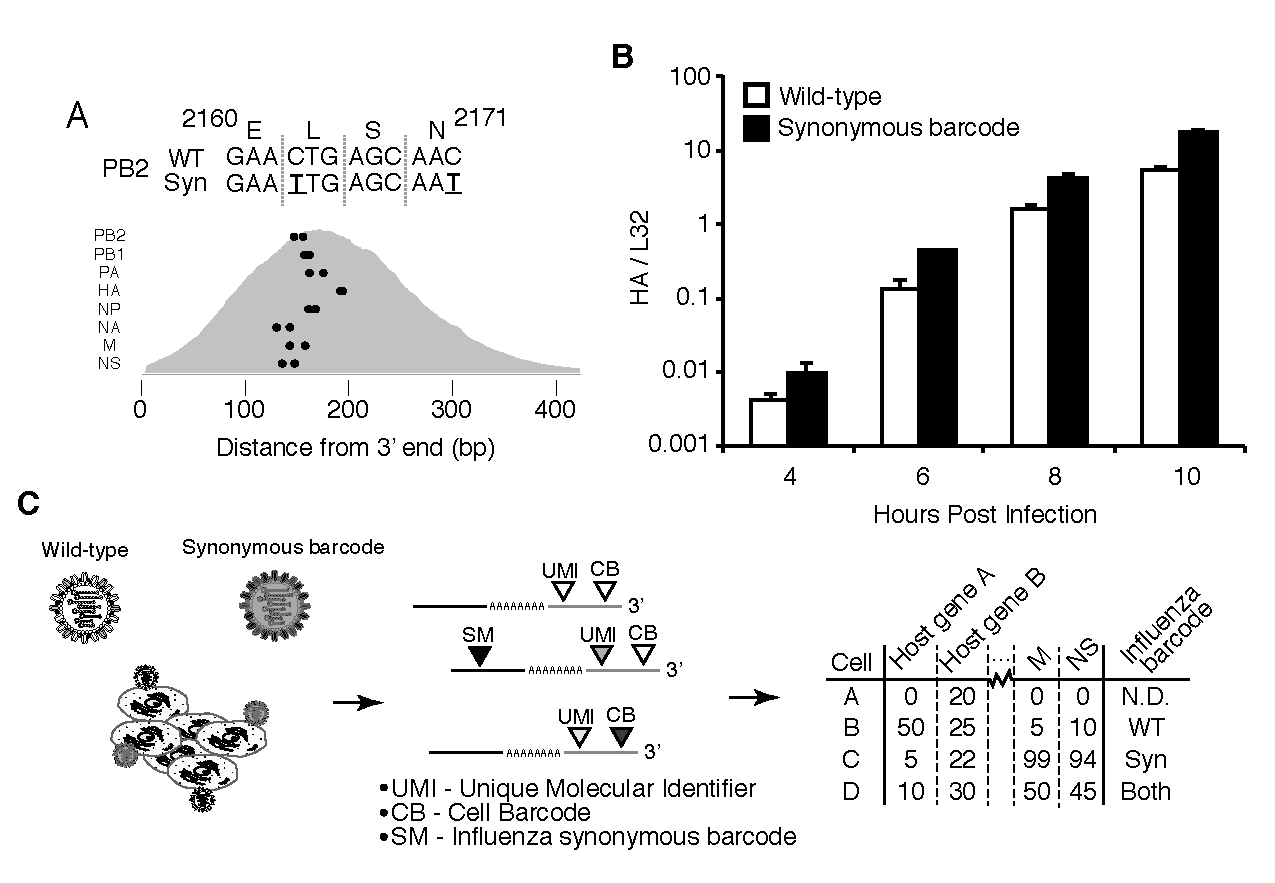
\includegraphics[width=0.8\linewidth]{figures/Workflow/workflow.pdf}}
\caption{\label{fig:workflow} Experimental design.
{\bf (A)}  
We engineered a virus that carried two synonymous mutations near the 3' end of each mRNA.
At top are the specific mutations for PB2.
At bottom are locations of the synonymous mutations relative to the typical distribution of read depth for our 3'-end sequencing.
{\bf (B)} 
The wild-type and synonymously barcoded viruses transcribe their genes with similar kinetics. 
Shown is the abundance of the viral hemagglutinin (HA) transcript relative to the cellular housekeeping gene L32 as assessed by qPCR in A549 cells infected at an MOI of 0.5 (as determined on MDCK-SIAT1 cells).
Error bars $\pm$ S.D., n=3.
{\bf (C)}  
A549 cells were infected with an equal mixture of mutant and wild-type virus. 
Immediately prior to collection, cells were physically separated into droplets and cDNA libraries were generated containing the indicated barcodes. 
The libraries were deep sequenced, and the data processed to create a matrix that gives the number of molecules of each transcript observed in each cell.
Infected cells were further annotated by whether their viral mRNAs derived from wild-type virus, synonymously barcoded virus, or both.
}
\figdata{Sequences of wild-type and barcoded viruses are in \texttt{viralsequences.fasta}.\label{figdata:viralsequences}}
\end{figure}

We took care to generate stocks of virus that were relatively ``pure'' of defective particles.
Stocks of viruses typically contain an array of biologically active viral particles, some of which are defective for replication owing to mutations or deletions in essential viral genes~\citep{von1954incomplete,huang1970defective,Brooke:2014ch,Fonville:2015cg,Lauring:2010if,Dimmock:2014dk}.
These defective particles become prevalent when a virus is grown at high multiplicity of infection (MOI), where complementation permits the growth of otherwise deleterious genotype.
To minimize the levels of defective particles, we propagated our viral stocks at low MOI for a relatively brief period of time~\citep{Xue:2016bw}.
We then validated that our stocks exhibited greater purity of infectious particles than a stock propagated at high MOI by verifying that they had a higher ratio of infectious particles to both virion RNA (Figure~\ref{fig:viruspopulations}A) and particles capable of inducing expression of a single viral protein (Figure~\ref{fig:viruspopulations}B).
In addition, viral stocks with many defective particles are more immunostimulatory~\citep{Tapia:2013kf,Lopez:2014en}.
We confirmed that our viral stocks induced much less interferon than a stock propagated at higher MOI (Figure~\ref{fig:viruspopulations}C).

\begin{figure}
\centerline{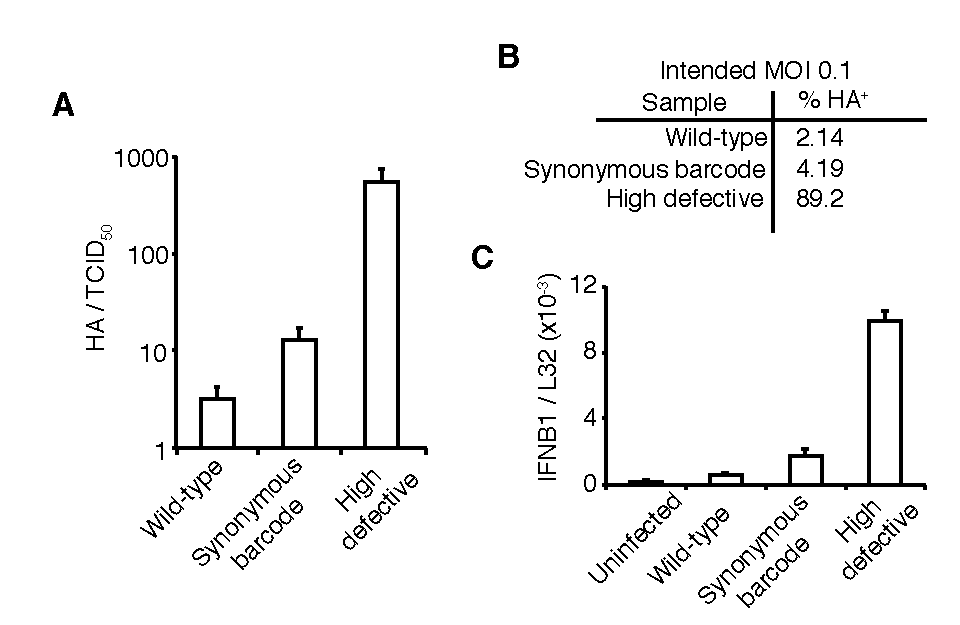
\includegraphics[width=0.7\linewidth]{figures/Validating_barcode_virus/validating_populations_D02.pdf}}
\caption{\label{fig:viruspopulations} The viral stocks in our experiments are relatively pure of defective particles. 
{\bf (A)}
Our viral stocks have a higher ratio of infectious particles to HA virion RNA compared to a high-defective stock propagated at high MOI.
HA viral RNA was quantified by qPCR on virions. 
Error bars $\pm$ S.D., n=6 (qPCR replicates). 
{\bf (B)} 
Our viral stocks have a higher ratio of infectious particles to particles capable of expressing the viral HA protein.
A549 cells were infected with all three viral stocks at an MOI of 0.1, and the percentage of cells expressing HA protein at 9 hours post-infection was quantified by antibody staining and flow cytometry.
{\bf (C)} 
Our viral stocks are less immunostimulatory than virus propagated at high MOI. 
Measurements of \textit{IFNB1} transcript by qPCR normalized to the housekeeping gene L32 in A549 cells at 10 hours post infection at an MOI of 0.5.
Error bars $\pm$ S.D., n=3.
Note that the MOIs were calculated by TCID50 on MDCK-SIAT1 cells, whereas the experiments in this figure involved infection of A549 cells.
}
\figsupp[Full flow cytometry data for panel B . \label{figsupp:HAstain}]{
Full flow cytometry date for  Figure~\ref{fig:viruspopulations}B. 
A549 cells were infected at an MOI of 0.1 as calculated by TCID50 on MDCK-SIAT1 cells. 
{\bf (A)} Uninfected gating control.
{\bf (B)} Cells infected with the wild-type virus stock used in our experiments.
{\bf (C)} Cells infected with synonymously barcoded virus stock used in our experiments.
{\bf (D)} Cells infected with a stock of wild-type virus propagated at a high MOI, and therefore enriched in defective particles.
}{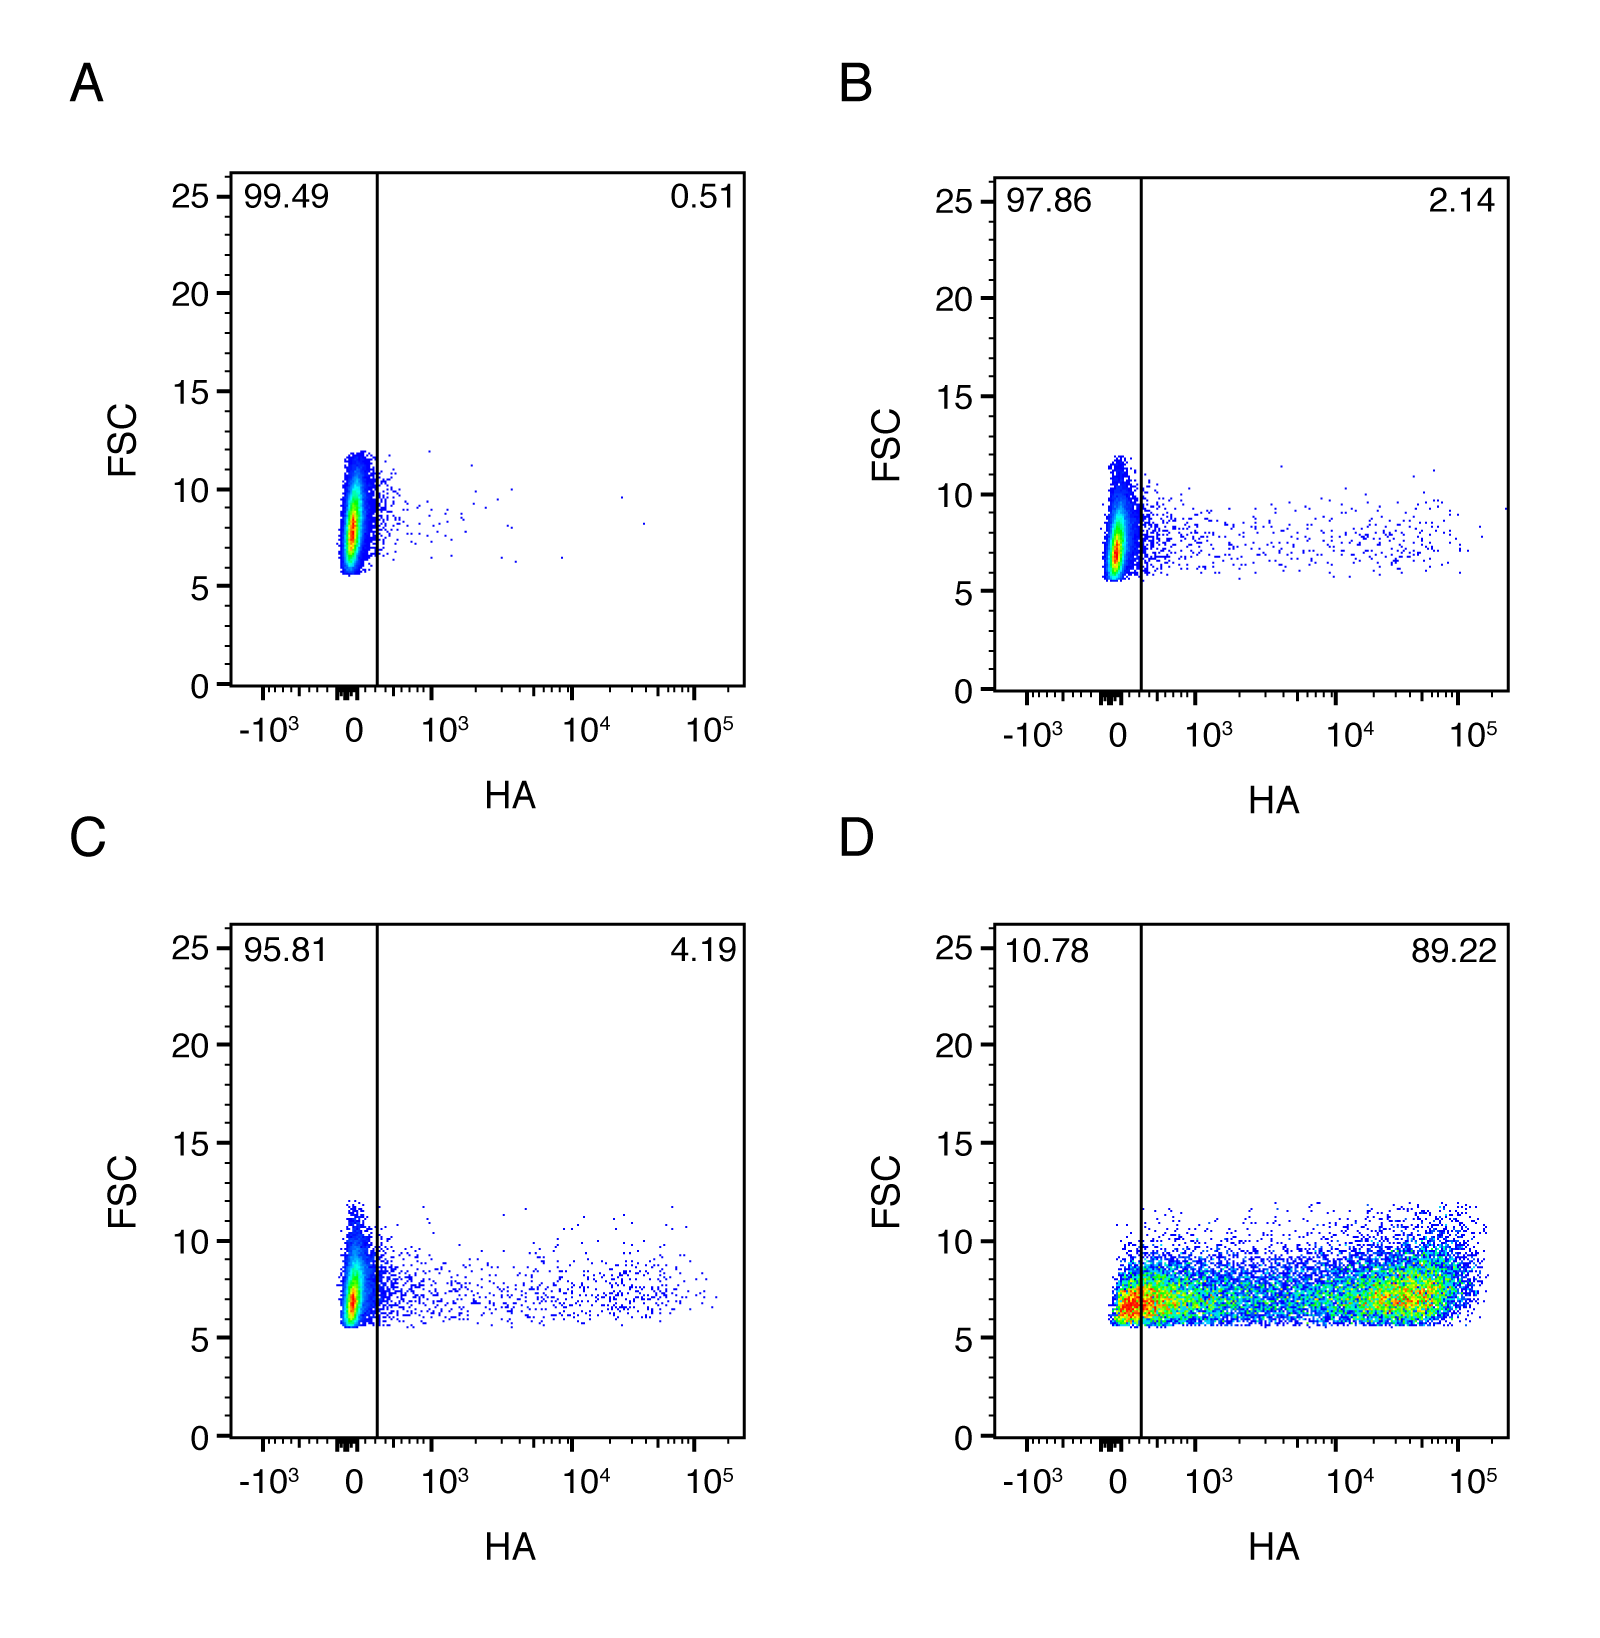
\includegraphics[width=0.7\linewidth]{figures/Validating_barcode_virus/HA_stain_supplement.png}}\end{figure}

\subsection{Single cells show an extremely wide range of expression of viral mRNA.}
We infected A549 cells at low MOI with a mixture of the wild-type and synonymously barcoded viruses, and collected cells for sequencing at 6, 8, and 10 hours post-infection, including a replicate of the 8-hour timepoint.
We recovered between 3,000 and 4,000 cells for each sample (Figure~\ref{fig:cells}A). 
As expected for a low-MOI infection, most cells expressed little or no viral mRNA (Figure~\ref{fig:cells}B).
Also as expected, the amount of viral mRNA per cell among infected cells increased over time (Figure~\ref{fig:cells}B).
But what was most notable was how widely the number of viral mRNA molecules varied among infected cells.
While the fraction of mRNA derived from virus was $<$0.1\% for most cells, viral mRNA constituted close to half the transcriptome in a few cells at 8 and 10 hours (Figure~\ref{fig:cells}C).
%Therefore, there is extraordinary variability in the number of viral transcripts per infected cell.

\begin{figure}
\centerline{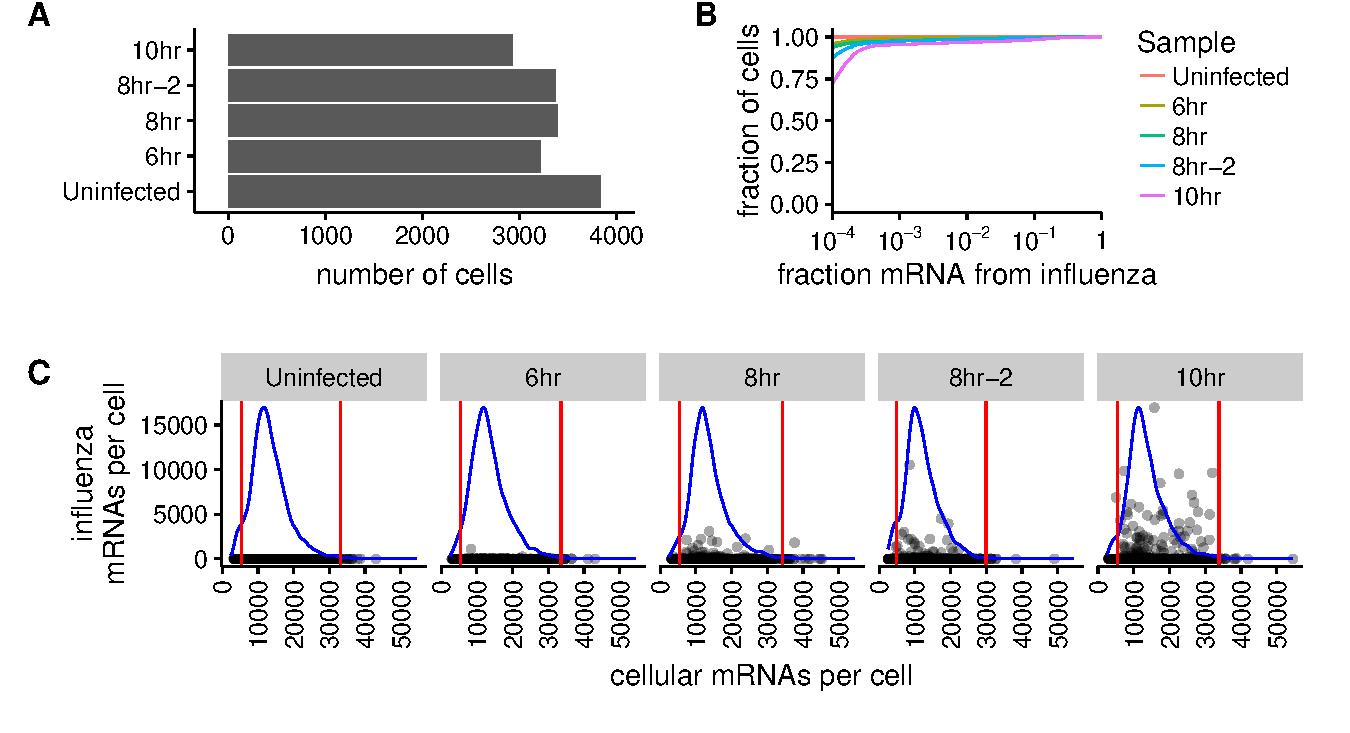
\includegraphics[width=0.9\linewidth]{figures/p_cell_mRNA_summary.pdf}}
\caption{\label{fig:cells}
There is a very wide distribution in the number of viral mRNAs detected per cell.
{\bf (A)} 
Number of cells sequenced for each sample.
{\bf (B)} 
Cumulative distribution of the fraction of mRNA derived from influenza virus for each sample.
For each point on the x-axis, the y-axis indicates the fraction of cells with at least that much of their mRNA from virus.
{\bf (C)} 
The number of cellular and viral mRNAs for each cell is plotted as a point.
The blue lines show the overall distribution of the number of cellular mRNAs per cell.
Cells outside the red lines were considered outliers (possibly derived from two cells per droplet), and were excluded from subsequent analyses.
}
\end{figure}

A complicating factor is that uninfected cells could have small amounts of viral mRNA due to leakage of transcripts from lysed cells.
It is therefore important to establish a threshold for identifying truly infected cells.
We can do this by taking advantage of the fact that roughly half the infecting virions bear synonymous barcodes.
Reads derived from lysed cells will be drawn from both wild-type and synonymously barcoded viral transcripts.
However, most cells are infected by at most one virion, and so the reads from truly infected cells will usually derive almost entirely from one of the two viral variants. 
Figure~\ref{fig:viralbarcodes}A shows the fraction of viral reads in individual cells from each viral variant, and Figure~\ref{fig:viralbarcodes}B indicates the fraction of viral reads from the most abundant variant in that cell.
Most cells with large amounts of viral mRNA have viral transcripts exclusively derived from one viral variant -- indicating non-random partitioning as expected from viral infection.
However, cells with a small amount of viral mRNA often have viral transcripts from both variants, as expected from the random partitioning associated with simple mRNA leakage.
Finally, a few cells with large amounts of viral mRNA have viral transcripts from both variants, reflecting co-infection with both variants.

We determined the threshold amount of viral mRNA per cell at which the barcode partitioning clearly resulted from infection rather than leakage (Figure~\ref{fig:viralbarcodes}C), and used this threshold to annotate cells that we were confident were truly infected.
We also annotated as co-infected cells above this threshold that had mRNA from both viral variants.
Figure~\ref{fig:viralbarcodes}D shows the number of cells annotated as infected and co-infected for each sample -- these cells are just a small fraction of the number of cells with any viral read.
These annotation thresholds are conservative, and will miss some true low-level infections, as well as any co-infections with the same viral variant.
However, it is important that the analyses below are restricted to cells that are truly infected with virus, so we accepted the loss of some low-level infections in order to avoid false positives.
Because the bulk of cells are not infected, we subsampled the uninfected cells to the numbers shown in Figure~\ref{fig:viralbarcodes}D to balance the proportions of infected and uninfected cells for all subsequent analyses.

Strikingly, the extreme variation in the number of viral transcripts per cell remains even after we apply these rigorous criteria for annotating infected cells (Figure~\ref{fig:viralbarcodes}E). 
The fraction of viral mRNA per infected cell follows a roughly exponential distribution, with many cells having few viral transcripts and a few cells having many.
In fact, a bare few infected cells contribute the majority of influenza transcripts.
Specifically, at 6 and 8 hours $<$10\% of infected cells are responsible for over half the viral transcripts, while at 10 hours $\approx$15\% of infected cells produce over half the viral transcripts (Figure~\ref{fig:viralbarcodes}-Figure~supplement~\ref{figsupp:cumulfracflu}).

\begin{figure}[t!]
\centerline{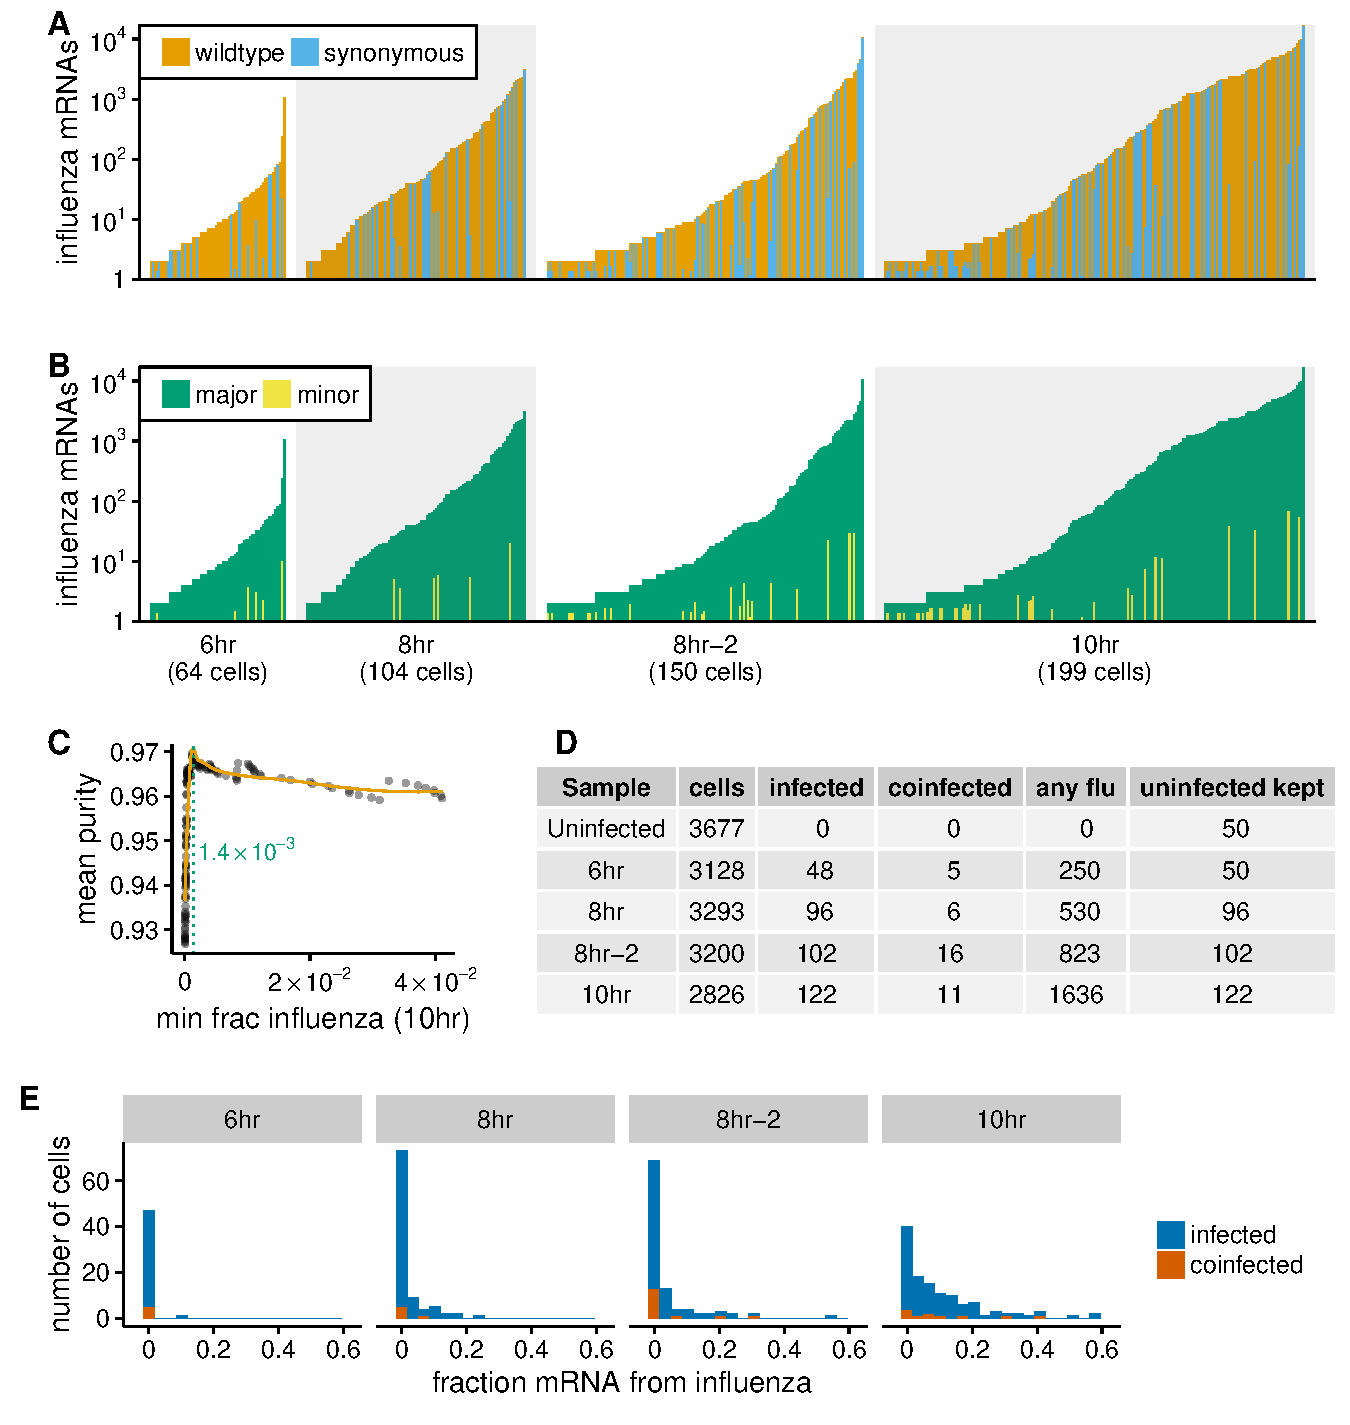
\includegraphics[width=0.9\linewidth]{figures/p_frac_flu_summary.pdf}}
\caption{\label{fig:viralbarcodes}
Synonymous barcodes on the viral mRNAs distinguish true infections from cells that contain viral mRNAs derived from leakage of lysed cells.
{\bf (A)}
Cells with at least two viral mRNAs for which the barcode could be called, arranged in order of increasing influenza transcript counts.
Bar heights denote the number viral mRNAs on a log\textsubscript{10} scale, bar coloring is linearly proportional to the fractions of viral mRNAs derived from wild-type and synonymously barcoded virus.
{\bf (B)}
Same as (A), but each bar is colored according to the relative fraction of the more common (major) and less common (minor) virus variant.
At low levels of viral mRNA there is often a roughly equal mix, suggesting contamination with viral mRNAs leaked from lysed cells.
At higher levels of viral mRNA, cells generally have only one viral variant, suggesting infection initiated by a single particle.
A few cells are also obviously co-infected with both viral variants.
{\bf (C)}
We determined a cutoff for calling ``true'' infections by fitting a curve to the mean barcode purity of all cells with greater than a given fraction of their mRNA derived from virus.
We called the cutoff at the point at which purity stops increasing with the fraction of viral mRNA.
{\bf (D)}
The number of cells identified as infected and co-infected for each sample, as well as the number of cells with any viral read.
For all subsequent analyses, we subsampled the number of uninfected cells per sample to the greater of 50 or the number of infected cells.
{\bf (E)} 
Distribution of the fraction of mRNA per cell derived from virus for both infected and co-infected cells.
}
\figsupp[Number of viral barcodes called.\label{figsupp:barcodescalled}]{
The number of viral barcodes called for each sample and influenza gene segment. 
Viral transcripts are classified as \emph{syn} if they mapped to a synonymously barcoded influenza transcript, \emph{wt} if they mapped to a wild-type influenza transcript, \emph{invalid} if multiple reads for the same UMI differed on the status of the viral barcode, and as \emph{uncalled} if none of the reads for that UMI overlapped the region of the viral transcript containing the viral barcode.
}{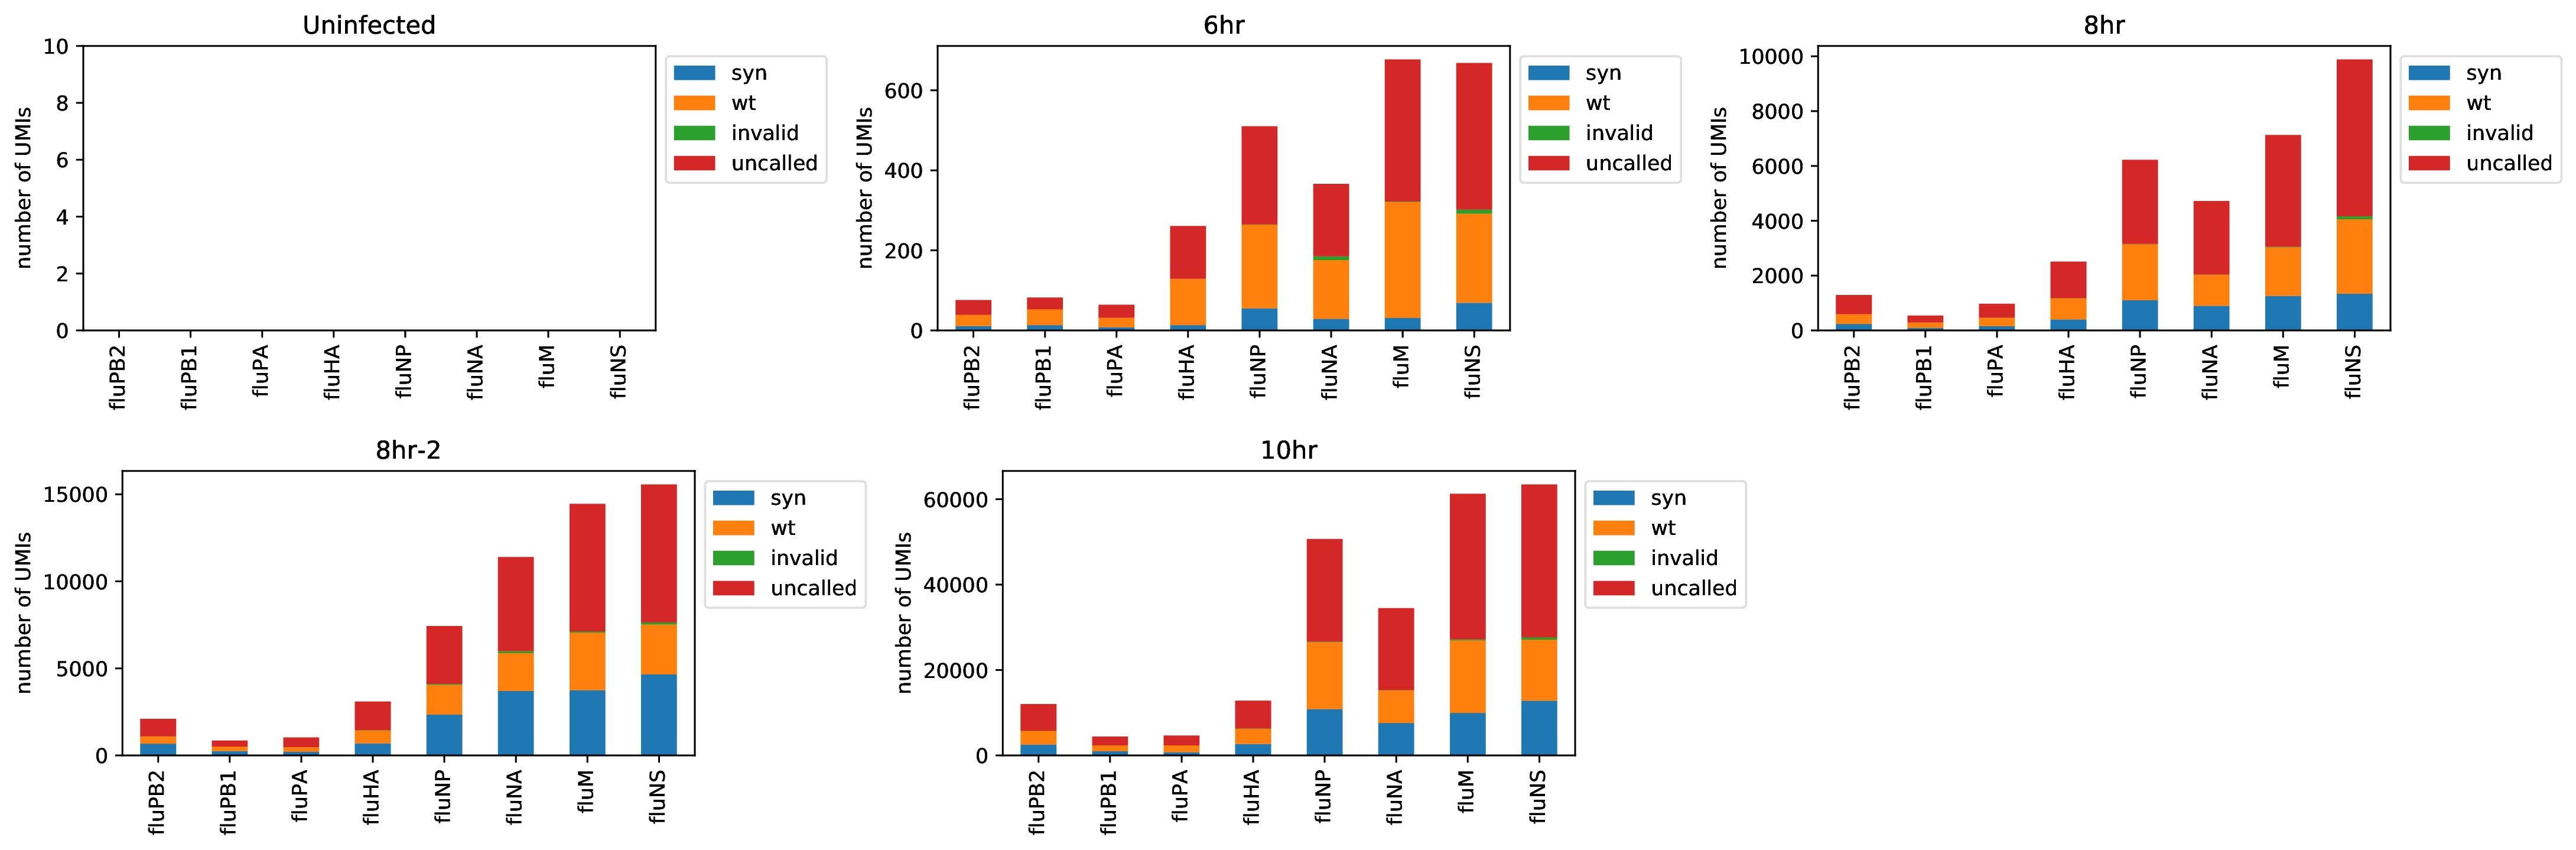
\includegraphics[width=\linewidth]{figures/synbarcodes_umistats.jpg}}
\figsupp[Fraction of total viral mRNA derived from a given fraction of infected cells.\label{figsupp:cumulfracflu}]{
The total fraction of all viral mRNA among infected cells that is attributable to a given fraction of these cells.
For instance, the plot for the 8-hour sample shows that roughly 50\% of all viral mRNA is derived from 10\% of the infected cells.
}{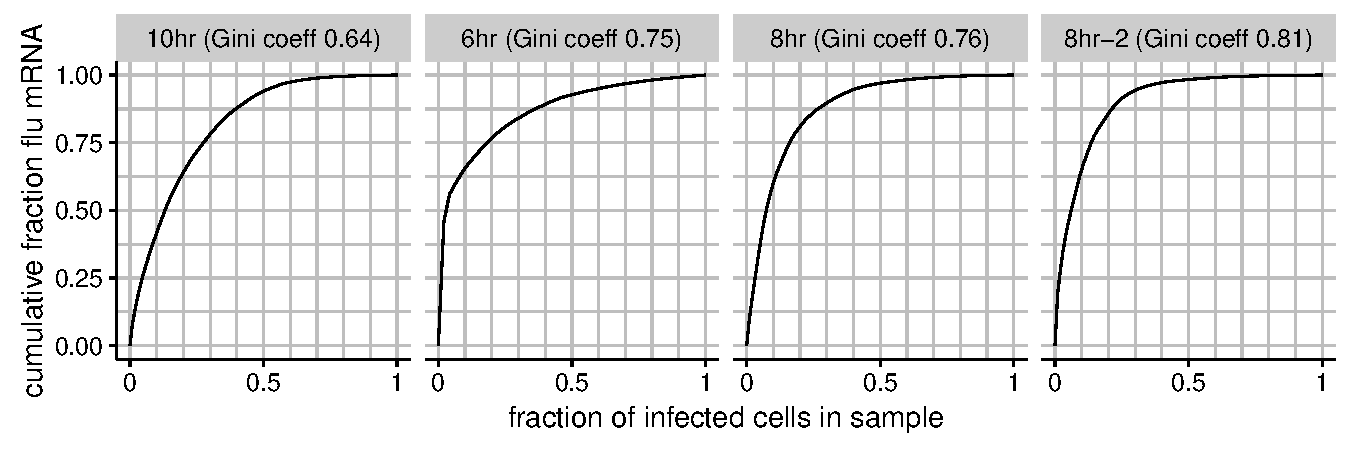
\includegraphics[width=\linewidth]{figures/p_cumul_flu.pdf}}
\end{figure}

\subsection{Absence of viral genes partially explains cell-to-cell variability in viral transcript abundance.}
The influenza genome is segmented, and cells can fail to express a viral mRNA if the encoding gene segment is not packaged in the infecting virion or fails to initiate transcription after infection.
Indeed, several groups have reported that the majority of infected cells fail to express at least one viral gene~\citep{Brooke:2013kb, Heldt:2015iz,Dou:2017cp}. 
We wondered if the absence of specific viral genes might be associated with reduced amounts of viral mRNA within single infected cells.
In particular, transcription of influenza virus mRNAs is performed by the viral ribonucleoprotein (RNP) complex, which consists of the three proteins that encode the tripartite polymerase (PB2, PB1, and PA) as well as nucleoprotein (NP)~\cite{huang1990determination}.
Each viral gene segment is associated with one RNP in incoming infecting virions, but secondary transcription by newly synthesized RNPs requires the presence of the viral genes for each of the four constituent RNP proteins so that the cell can produce more RNP proteins~\citep{Vreede:2004ip,eisfeld2015centre}.
This secondary transcription is a major source of viral mRNAs, as evidenced by the fact that blocking synthesis of the RNP proteins reduces the amount of viral mRNA by several orders of magnitude in bulk cells (Figure~\ref{fig:fluburdenbyflugene}-Figure~supplement~\ref{figsupp:cyclohexamide}).

\begin{figure}[t!]
\centerline{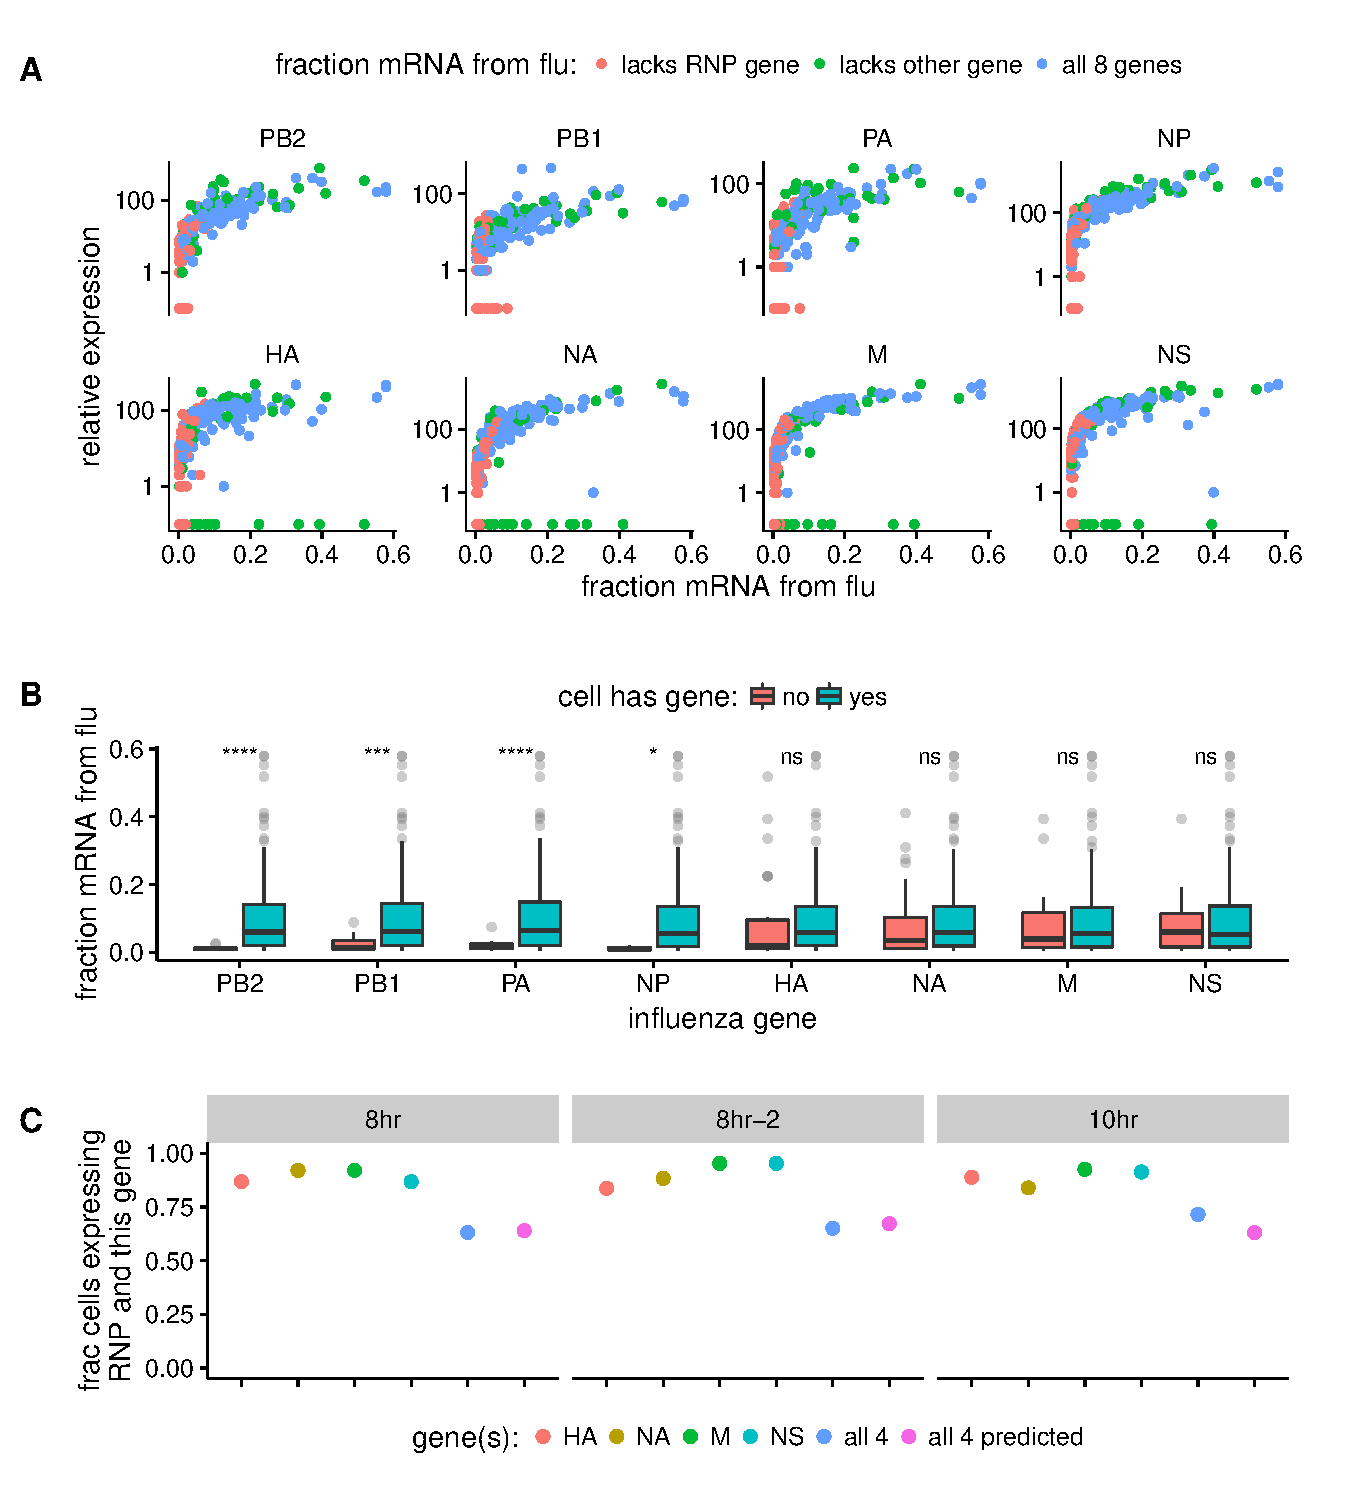
\includegraphics[width=0.9\linewidth]{figures/p_flu_burden_flu_gene_merge.pdf}}
\caption{\label{fig:fluburdenbyflugene}
The absence of viral genes explains some of the variability in the amount of viral mRNA per cell.
{\bf (A)} 
Fraction of mRNA in each infected cell derived from virus as a function of the normalized expression of each viral gene in that cell, taken over all time points.
Cells with high viral burden always express all the RNP genes, but some cells with high viral burden lack each of the other viral genes.
{\bf (B)}
Box plots showing the per-cell viral burden among cells with $>$0.5\% of their mRNA from virus, binned by whether or not the cells express each viral gene.
A Wilcoxon signed-rank test was used to test the null hypothesis that absence of each gene does not affect viral burden: **** = $P < 10^{-4}$, *** = $P < 10^{-3}$,  * = $P < 0.05$, ns = not significant.
Similar results are obtained if we examine only the 10-hour timepoint (Figure~\ref{fig:fluburdenbyflugene}-Figure~supplement~\ref{figsupp:10hrfluburdenbyflugene}).
Top and bottom of box bound the first and third quartiles; the line in the box is at the median.
Whiskers extend to the highest or lowest point within1.5$\times$ the interquartile range, and outliers are shown as circles.
{\bf (C)}
Among cells that express all four RNP genes, this panel shows the fraction of that express each of the four other genes, as well as the fraction that express \emph{all} four of the other genes.
The fraction that express all four other genes is well predicted by simply multiplying the frequencies of cells that express each of these genes individually, indicating that gene absence is approximately independent across these four genes.
}
\figsupp[Secondary transcription from newly synthesized RNPs is a major source of viral mRNA during bulk infections.\label{figsupp:cyclohexamide}]{
A549 cells were infected at an MOI of 0.2 as calculated on MDCK-SIAT1 cels in either the presence or absence of the protein-translation inhibitor cyclohexamide, and viral mRNA was quantified at 8 hours post-infection by qPCR.
The cyclohexamide prevents translation of new PB2, PB1, PA, and NP protein, and so prevents the formation of the new RNPs needed for secondary transcription.
The bars show the relative amount of HA and PB2 mRNA in the absence versus the presence of cyclohexamide. Error $\pm$ S.D. n=3. 
}{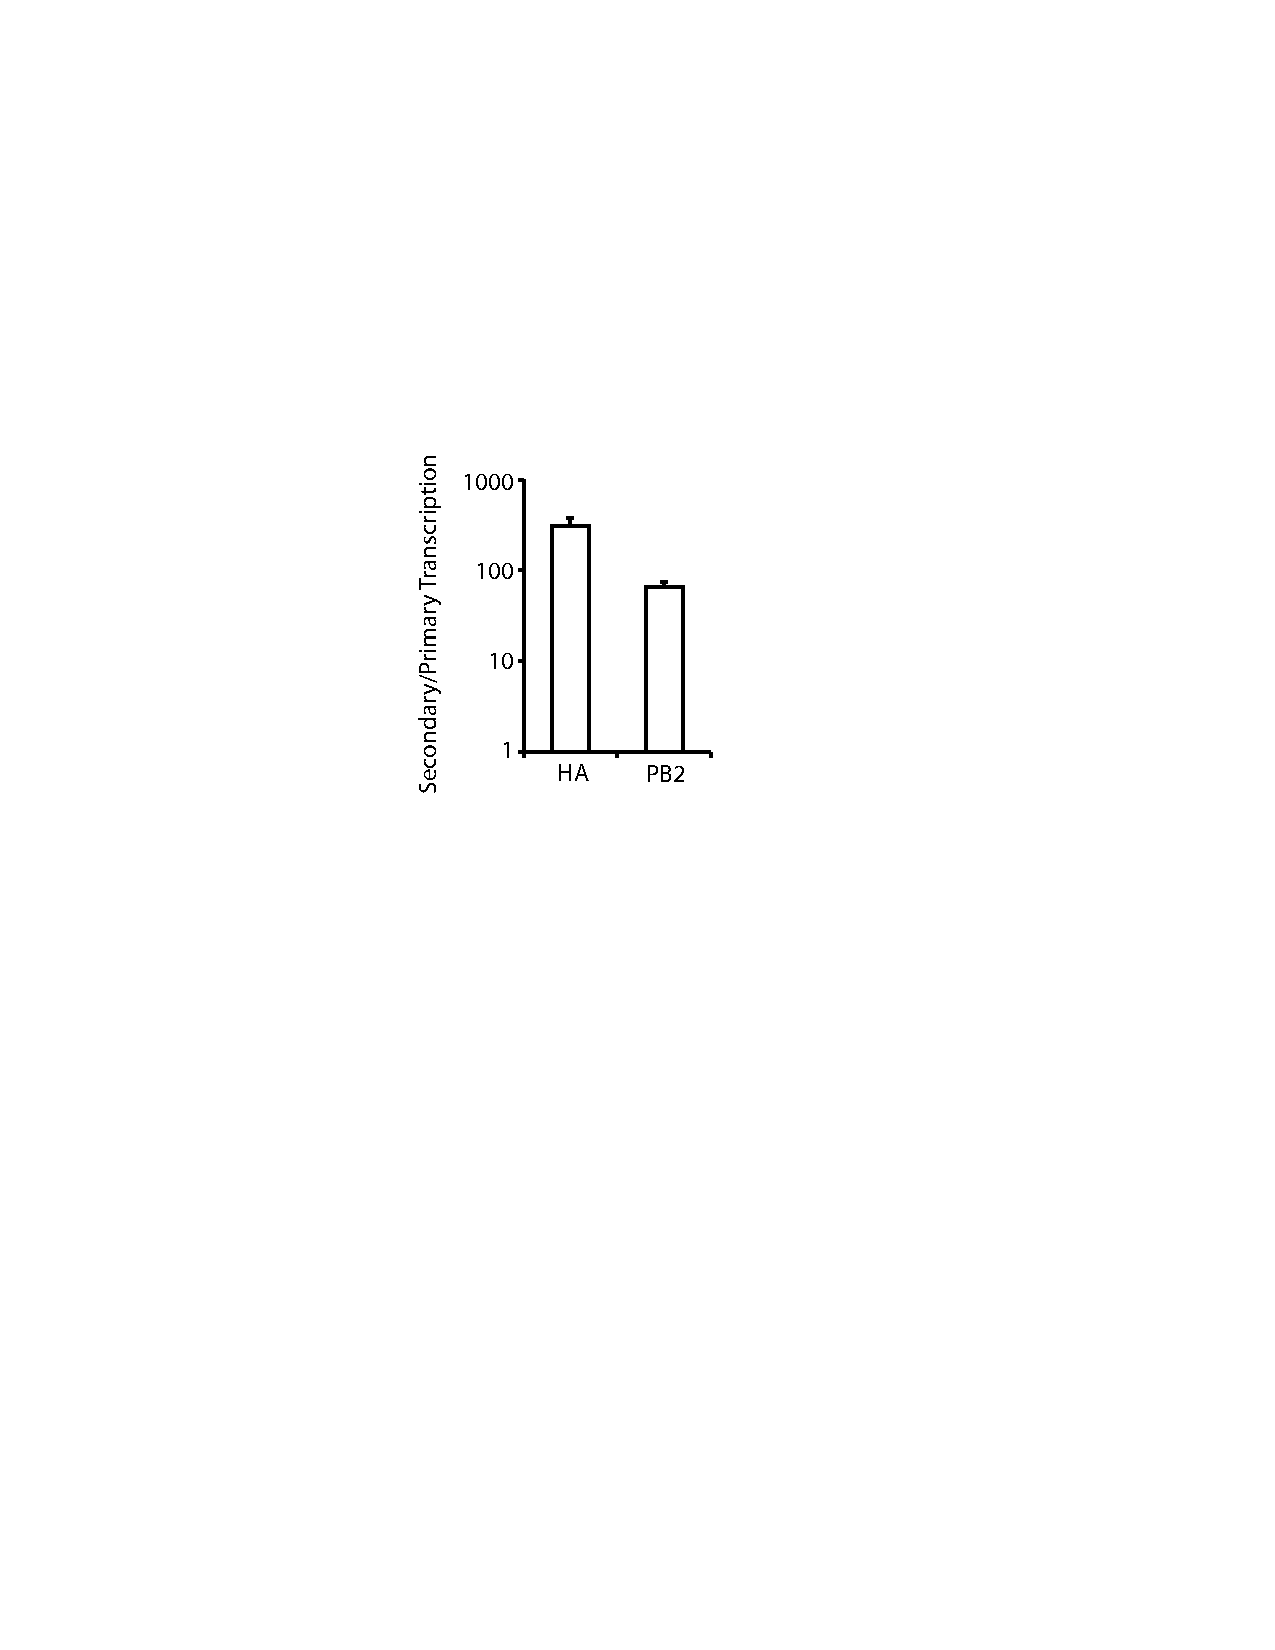
\includegraphics[width=0.3\linewidth]{figures/Primary_transcription_measurements/Cyclohexamide.pdf}}
\figsupp[Like panel (B) but for the 10-hr sample only.\label{figsupp:10hrfluburdenbyflugene}]{
The absence of viral RNP genes but \emph{not} non-RNP genes remains significantly associated with reduced viral burden when we examine only the 10-hr sample, which is the single time point with the most data points.
The difference for NP is no longer statistically significant due to low counts of infected cells lacking NP, but the trend remains.
}{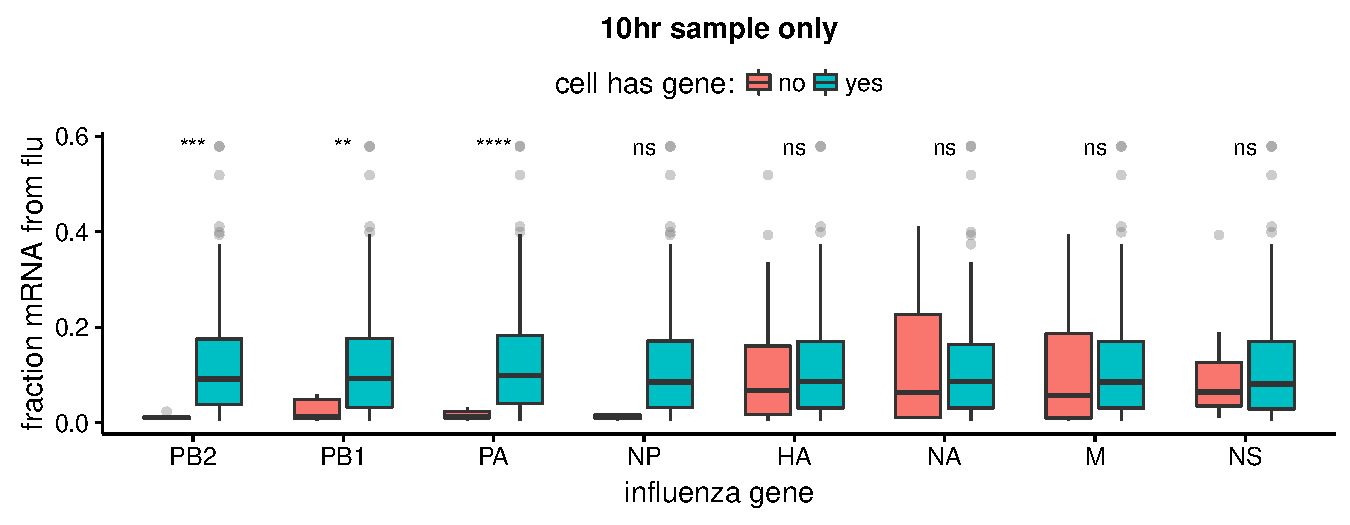
\includegraphics[width=\linewidth]{figures/p_10hr_flu_burden_flu_gene_test}}
\figdata{The numerical data for panel (C) are in \texttt{p\_missing\_genes.csv}.}
\end{figure}

We examined the total amount of viral mRNA versus the expression of each viral gene (Figure~\ref{fig:fluburdenbyflugene}A). 
Cells that lack an RNP gene never derive more than a few percent of their mRNAs from virus, confirming the expected result that all four RNP genes are essential for high levels of viral transcription.
However, we observe cells that lack each of the other non-RNP genes but still derive $\approx$40\% of their mRNAs from virus, suggesting that none of the other genes are important for high levels of viral transcription.
These results are statistically supported by Figure~\ref{fig:fluburdenbyflugene}B, which shows that absence of any RNP gene but \emph{not} any other viral gene is associated with reduced amounts of viral mRNA. 
However, gene absence clearly does not explain all of the variability in viral gene expression, since even cells expressing all viral genes exhibit a very wide distribution in the amount of viral mRNA that they express. 
The rest of this variability must be due to additional mechanisms such as differences in host-cell state, viral mutations not detectable by our 3'-end sequencing approach, or inherent stochasticity.  

We also sought to quantify the fraction of infected cells that completely failed to express a given gene.
We limited this analysis to examining the presence / absence of the non-RNP genes in cells expressing all four RNP genes, since we might fail to detect viral transcripts that are actually present at low levels in RNP-deficient cells due to the lower viral burden in these cells.
At the 8- and 10-hour time points, between 5\% and 17\% of cells fail to express any one of the four non-RNP genes (Figure~\ref{fig:fluburdenbyflugene}C).
The absence of a given gene appears to be an independent event, as the probability of observing all four non-RNP genes in a cell is well predicted by simply multiplying the probabilities of observing each gene individually (Figure~\ref{fig:fluburdenbyflugene}C). 
Our measurements of the frequency at which infected cells fail to express individual viral genes are roughly consistent with estimates made by others using different means~\citep{Brooke:2013kb,Dou:2017cp}.
	
\subsection{The relative amounts of different viral mRNAs are fairly consistent across cells.}
The results above show that the total amount of viral mRNA in infected cells varies over orders of magnitude.
Does the relative expression of viral genes exhibit similar cell-to-cell variability?
To address this question, we focused on cells that derived $>$5\% of their mRNA from virus, since estimates of relative viral gene expression will be less noisy in cells with more viral mRNAs.

\begin{figure}
\centerline{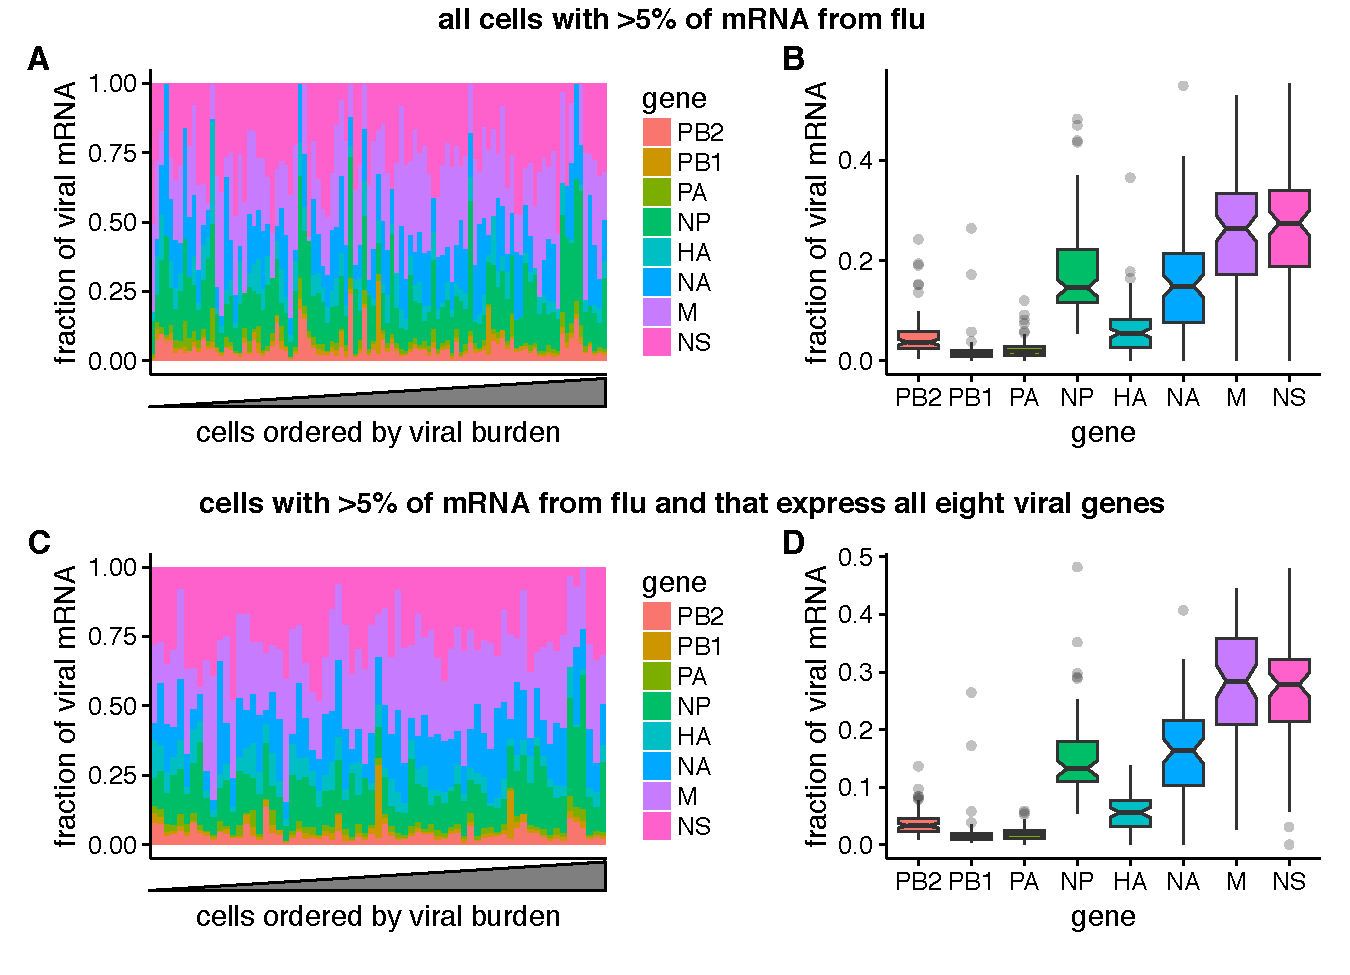
\includegraphics[width=0.9\linewidth]{figures/p_flu_expr_aledit.pdf}}
\caption{\label{fig:fluexpr}
Relative expression of influenza virus genes in highly infected cells (>5\% of total mRNA from virus).
{\bf (A)} 
The fraction of viral mRNA from each viral gene for each cell. 
{\bf (B)}
Box plots showing the distribution of the fraction of viral mRNA per cell from each viral gene.
The black lines at the notches are the medians, and the tops and bottoms of boxes indicate the first and third quartiles.
Whiskers extend to the highest or lowest data point observed within 1.5x the interquartile range, outliers shown as circles.
Notches extend 1.58x the interquartile range divided by the square root of the number of observations. 
{\bf (C)}, {\bf (D)} 
The same plots, but only including cells for which we observed at least one molecule of each viral gene.
}
\figdata{The raw data are in \texttt{p\_flu\_expr.csv}.}
\end{figure}

In contrast to the extreme variability in the total viral mRNA per cell, the fraction of this mRNA derived from each gene is much more consistent across cells (Figure~\ref{fig:fluexpr}A).
Total viral mRNA varies by orders of magnitude, but the fraction from any given viral gene is fairly tightly clustered around the median value for all cells (Figure~\ref{fig:fluexpr}B).
The relative levels of each viral mRNA in our cells are similar to prior bulk measurements made by Northern blots~\citep{Hatada:1989vz}, which also found an expression hierarchy of M $>$ NS $\gg$ NP $>$ NA $>$ HA $\gg$ PB2 $\sim$ PB1 $\sim$ PA.
The cell-to-cell consistency in the relative expression of different viral genes generally becomes even tighter if we limit the analysis only to cells that express all eight viral genes (Figure~\ref{fig:fluexpr}C,D).
Therefore, with the exception of complete gene absence, the factors that drive the dramatic cell-to-cell variability in the amount of viral mRNA appear to have roughly similar effects on all viral genes in a given cell.
This finding is consistent with prior work showing positive correlations among the abundance of several viral gene segments in individual cells ~\citep{Heldt:2015iz}.

\subsection{Co-infection can provide infected cells with the full complement of viral genes.}
Our sequencing enables us to identify the rare cells that were co-infected with both wild-type and synonymously barcoded viral variants.
Overall, we captured 10 such co-infected cells that had $>$5\% of their mRNA derived from virus (Figure~\ref{fig:coexpression}).
Seven of these 10 cells expressed all eight viral genes.
Remarkably, the majority (4 of 7) of these cells would \emph{not} have expressed all the viral genes in the absence of co-infection, since they have at least one gene exclusively derived from each viral variant.
For instance, the cell with 11.2\% of its mRNA from virus in the upper right of Figure~\ref{fig:coexpression} expresses M only from the wildtype viral variant, and NP and HA only from the synonymously barcoded variant.
Our data therefore provide direct single-cell support for the idea that co-infection can rescue missing viral genes~\citep{Brooke:2013kb,Fonville:2015cg,aguilera2017plaques}.

\begin{figure}
\centerline{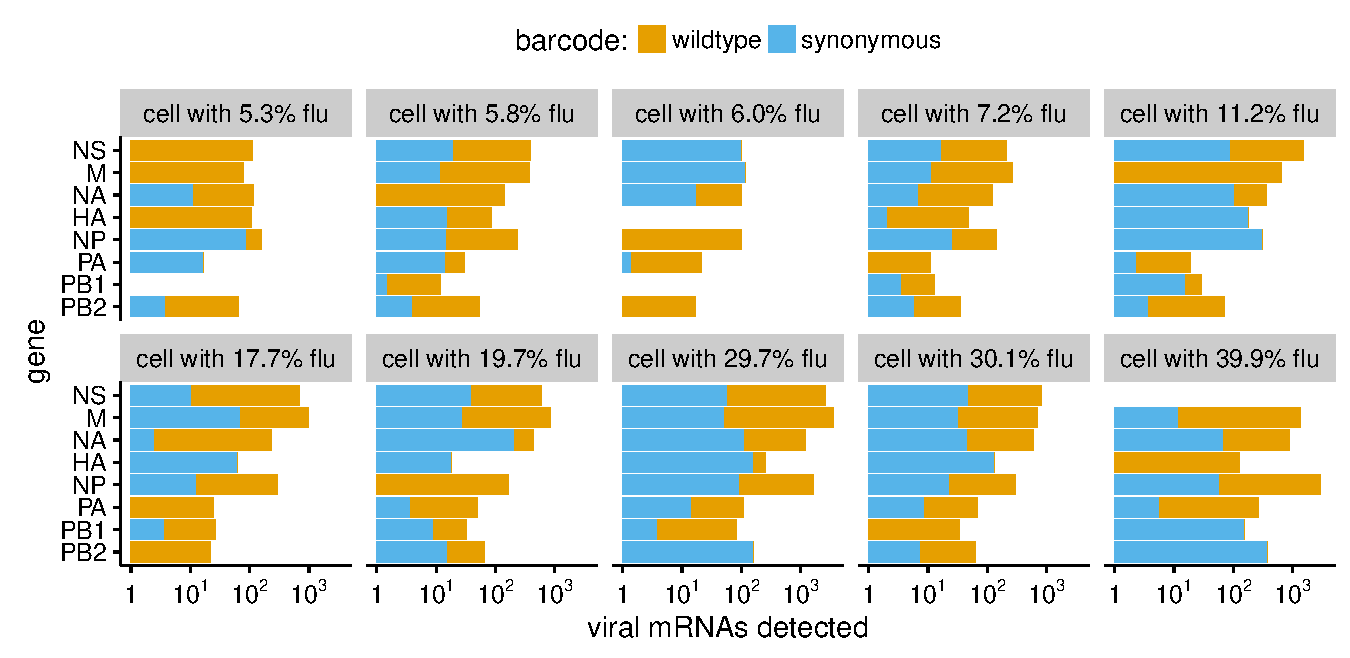
\includegraphics[width=0.9\linewidth]{figures/p_coinfection.pdf}}
\caption{\label{fig:coexpression}
The abundance of each viral transcript in cells that are co-infected with the two viral variants and have $>$5\% of their mRNA derived from virus.
The bars show the logarithms of the numbers of each viral mRNA detected, and are colored in linear proportion to the fraction of that mRNAs derived from wild-type or synonymously barcoded virus.
}
\figsupp[Co-infected cells express roughly equal amounts of a gene from each infecting viral variant. \label{figsupp:flowcyto}]{
{\bf(A)} Cells were co-infected with a mix of wild-type virus and virus in which the HA gene was replaced by GFP flanked by the terminal regions of the HA gene segment. 
At 10 hours post-infection, cells were analyzed by flow cytometry for HA and eGFP expression.
{\bf(B)} The expression of HA and GFP are correlated in co-infected cells. 
Shown are the quantile-normalized HA and eGFP signals for double-positive cells. 
Cells are colored by density, using a Gaussian kernel density estimate. 
{\bf(C)},{\bf(D)},{\bf(E)} Gating controls, single infection with eGFP virus, single infection with wild-type virus, and uninfected cells, respectively. 
{\bf(F)} Gaussian kernel density estimate on HA positive cells from {\bf(C)}
}{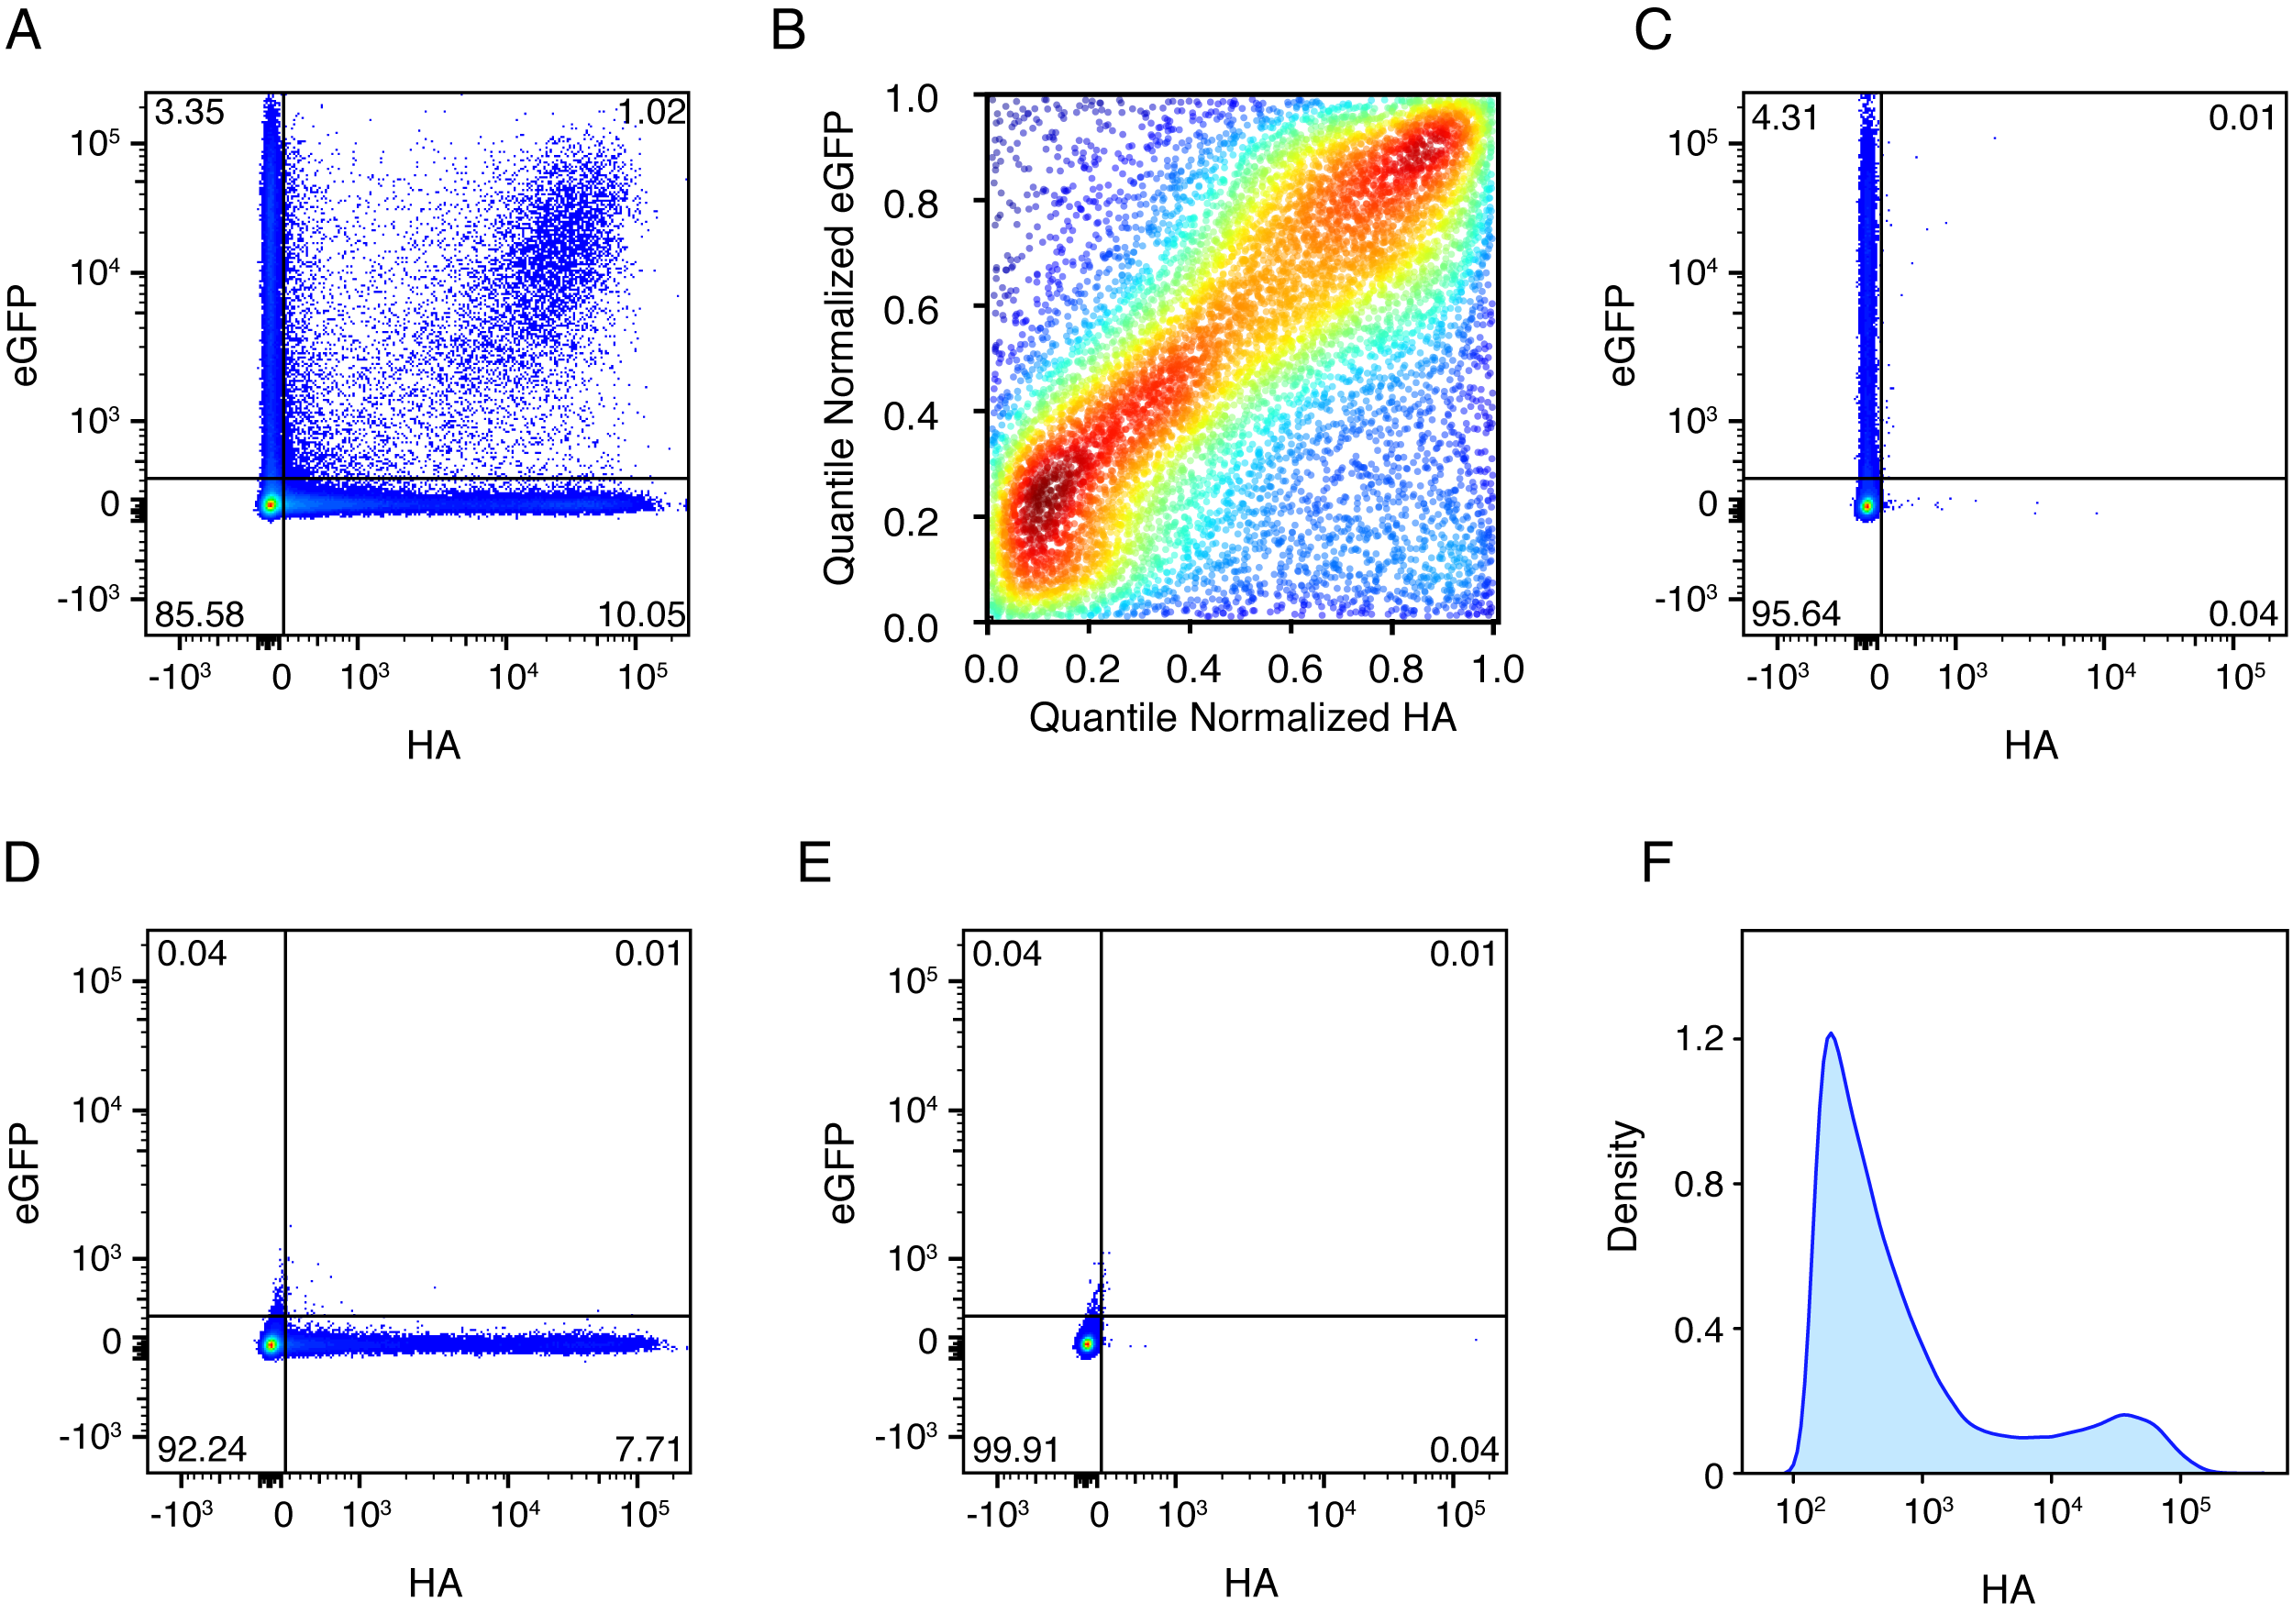
\includegraphics[width=\linewidth]{figures/Pseudovirus_flow_cytometry/coinfFlow_D03.png}}
\figdata{The raw data plotted in this figure are in \texttt{p\_co-infection.csv}.}
\figdata{The sequence of the HA viral RNA carrying the GFP gene is in \texttt{HAflank-eGFP.fasta}.\label{figdata:HAflank}}
\end{figure} 
Another observation from Figure~\ref{fig:coexpression} is that co-infected cells usually express roughly equal amounts of transcripts from each of the two viral variants.
This observation is consistent with the finding by \citet{Dou:2017cp} and \citet{Huang:2008gy} that the temporal window for co-infection is short -- if both viral variants infect a cell at about the same time, then neither will have a headstart and so each will have a roughly equal opportunity to transcribe its genes.

To support this idea with a larger dataset albeit at lower resolution, we generated a virus in which the HA coding sequence was replaced by GFP.
We then co-infected cells with a mix of wildtype and $\Delta$HA-GFP virus and used flow cytometry to score cells for the presence of HA only (infection by wildtype virus), GFP only (infection by $\Delta$HA-GFP virus), or both (co-infection) as shown in Figure~\ref{fig:coexpression}~Figure~supplement~\ref{figsupp:flowcyto}.
As in our single-cell sequencing data, we found that expression of HA and GFP were highly correlated, indicating that co-infected cells typically expressed roughly equal amounts of transcript from each viral variant.

\subsection{Activation of the interferon response is rare in single infected cells.}
Because our sequencing captured all polyadenylated transcripts, we can examine whether there are prominent changes in the host-cell transcriptome in sub-populations of infected cells.
In particular, influenza virus infection can trigger innate-immune sensors that lead to the transcriptional induction of type I and III interferons, and subsequently of anti-viral interferon-stimulated genes~\citep{Killip:2015dw,Iwasaki:2014dw,Crotta:2013ef}.
In bulk cells, this interferon response is one of the most prominent transcriptional signatures of influenza-virus infection~\citep{Geiss:2002a}.
However, activation of the interferon response is stochastic and bi-modal at the level of single cells~\citep{Chen:2010cr,Shalek:2014ey,Shalek:2013ej,PerezCidoncha:2014jr,bhushal2017cell}.
We therefore hypothesized that we might see two sub-populations of infected cells: one in which the interferon response inhibited viral transcription, and another in which the virus was able to express high levels of its mRNA by evading or blocking this response.

\begin{figure}
\centerline{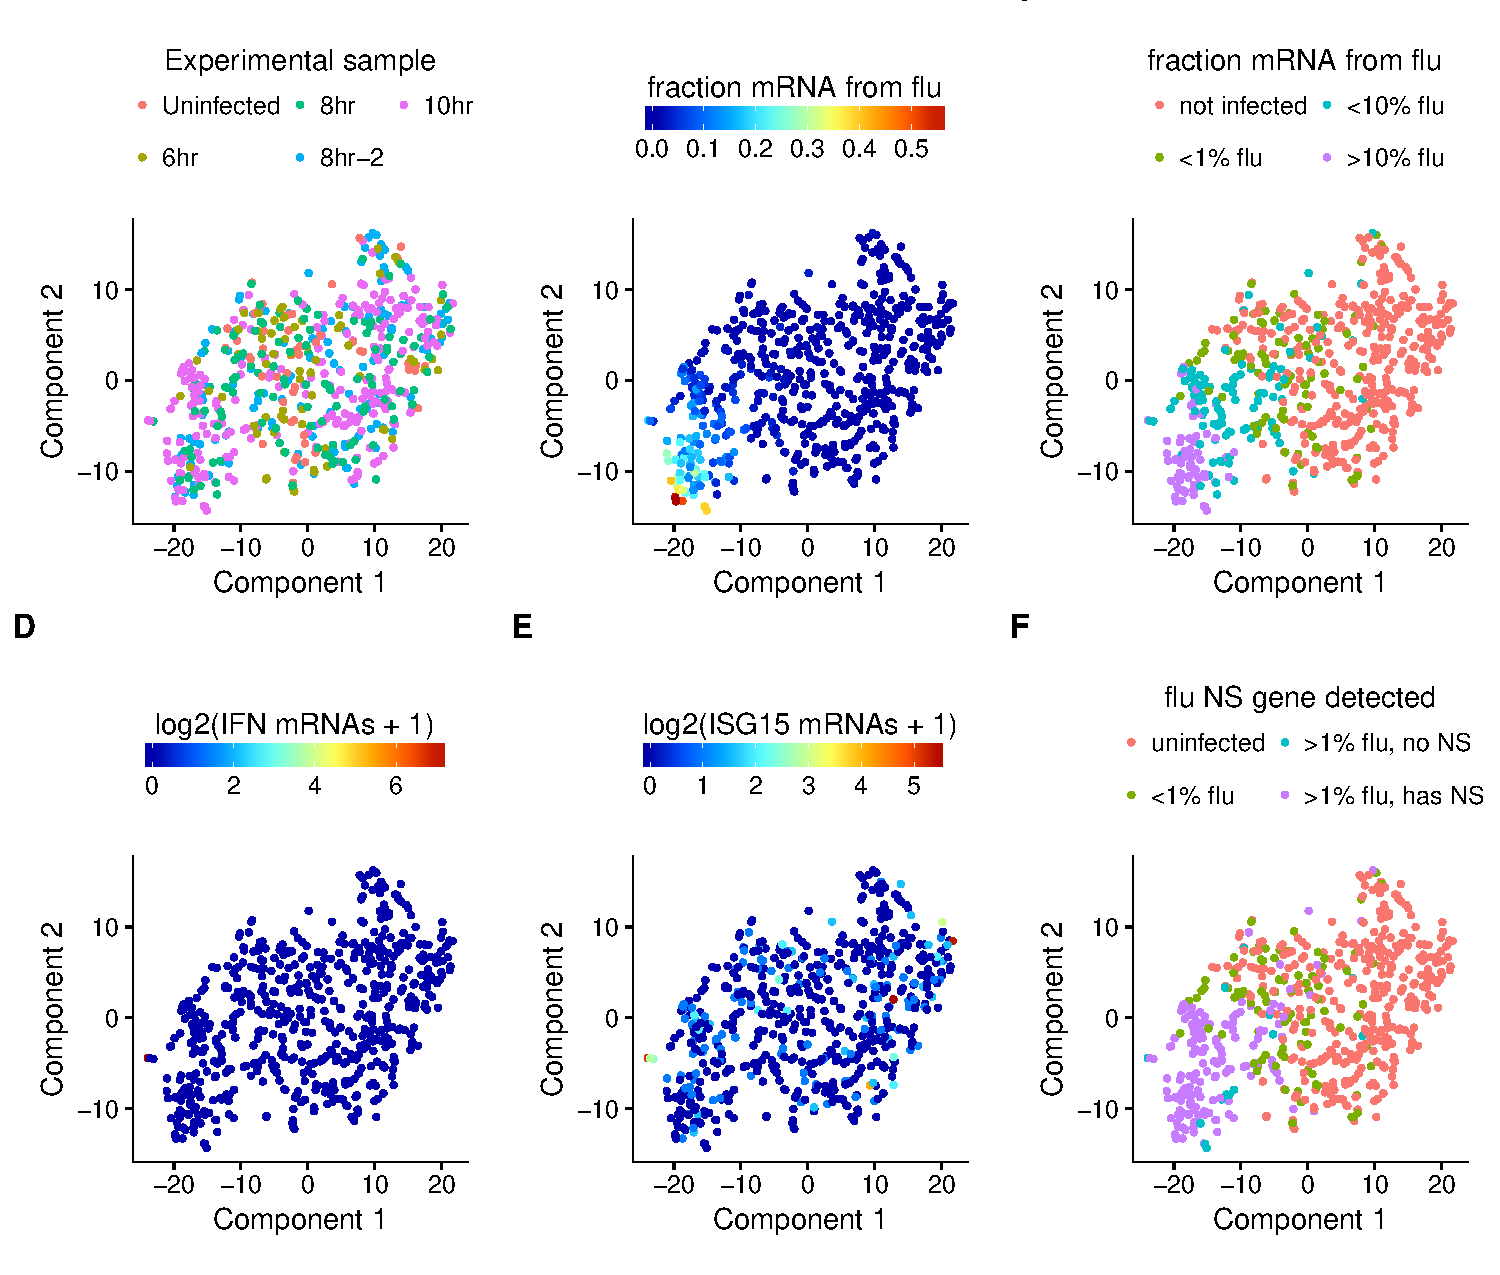
\includegraphics[width=0.8\linewidth]{figures/p_small_tsne_merge.pdf}}
\caption{\label{fig:tsne}
A t-SNE plot created by semi-supervised clustering of the cells using genes that co-vary with viral infection status.
Each point is a single cell, and each panel shows an identical layout but colors the cells according to a different property.
{\bf (A), (B)}
Cells colored by the fraction of their mRNA that is derived from virus.
{\bf (C)}
Cells colored by the experimental sample from which they are derived.
{\bf (D), (E)}
Cells colored by the number of detected transcripts from type I and III interferons (IFN).
Only one cell has detectable interferon expression.
{\bf (E)}
Cells colored by the expression of the interferon-stimulated gene IFIT1.
{\bf (F)}
Cells colored by whether they express the viral NS gene.
The one interferon-positive cell is lacking NS, but many interferon-negative cells also lack NS.
}

\end{figure}

To examine whether there were distinct sub-populations of virus-infected cells, we used a semi-supervised t-SNE approach~\citep{VanderMaaten:2008tm} to cluster cells by genes that co-varied with viral infection status.
As shown in Figure~\ref{fig:tsne}A,B, this approach effectively grouped cells by the amount of viral mRNA that they expressed.
Sample-to-sample variation was regressed away during the clustering, as cells did not obviously group by time-point, with expected exception that the uninfected and 6-hour samples had few cells in the region of the plot corresponding to large amounts of viral mRNA (Figure~\ref{fig:tsne}C).

But to our surprise, we did not see a prominent clustering of infected cells into sub-populations as expected if the interferon response was strongly activated in some cells.
To investigate further, we annotated each cell by the total number of type I and III interferon transcripts detected.
Remarkably, only a single cell expressed detectable interferon (Figure~\ref{fig:tsne}D).
We also examined interferon-stimulated genes, which are induced by autocrine and paracrine interferon signaling.
Figure~\ref{fig:tsne}E shows expression of one such gene, IFIT1~\citep{Fensterl:2011fp}.
As with interferon itself, expression of IFIT1 was rare and most prominent in the single interferon-positive cell, presumably due to the higher efficiency of autocrine versus paracrine signaling.
Notably, interferon and interferon-stimulated genes were also relatively ineffective at blocking viral transcription in the single cell in which they were potently induced, since $>$10\% of the mRNA in this cell was derived from virus (Figure~\ref{fig:tsne}A,B,D,E).

We posited that the paucity of interferon induction might be due to the activity of influenza virus's major interferon antagonist, the NS1 protein.
We therefore identified cells that expressed substantial amounts of viral mRNA but lacked the NS gene (Figure~\ref{fig:tsne}F).
Consistent with the idea that NS1 is important for suppressing interferon, the one interferon-positive cell lacked detectable expression of the NS gene.
But other cells that lacked NS expression still failed to induce a detectable interferon response, despite often having $>$10\% of their mRNA derived from virus (Figure~\ref{fig:tsne}).
Therefore, most infected cells fail to express interferon even when the virus lacks its major known interferon antagonist.
Our results are in line with other work showing that NS1-deficient influenza virus fails to deterministically induce interferon~\citep{Killip:2017ef,Kallfass:2013kp}.
Therefore, single cells infected at low MOI with a relatively ``pure'' stock of influenza virus clearly activate innate-immune responses much less frequently than might be presumed from bulk studies that flood cells with viral stocks full of defective particles.

\subsection{Genes involved in the oxidative-stress response co-vary with viral gene expression.}
We examined whether any host genes were differentially expressed in cells with more viral mRNA.
We restricted this analysis to infected cells with all eight viral genes in order to focus on cellular genes that were associated with viral mRNA burden independent of any effects due to the stochastic presence or absence of particular viral transcripts.
We identified 45 cellular genes that co-varied with viral gene expression at a false discovery rate of 0.1 (Figure~\ref{fig:cellulargenes}).

\begin{figure}
\centerline{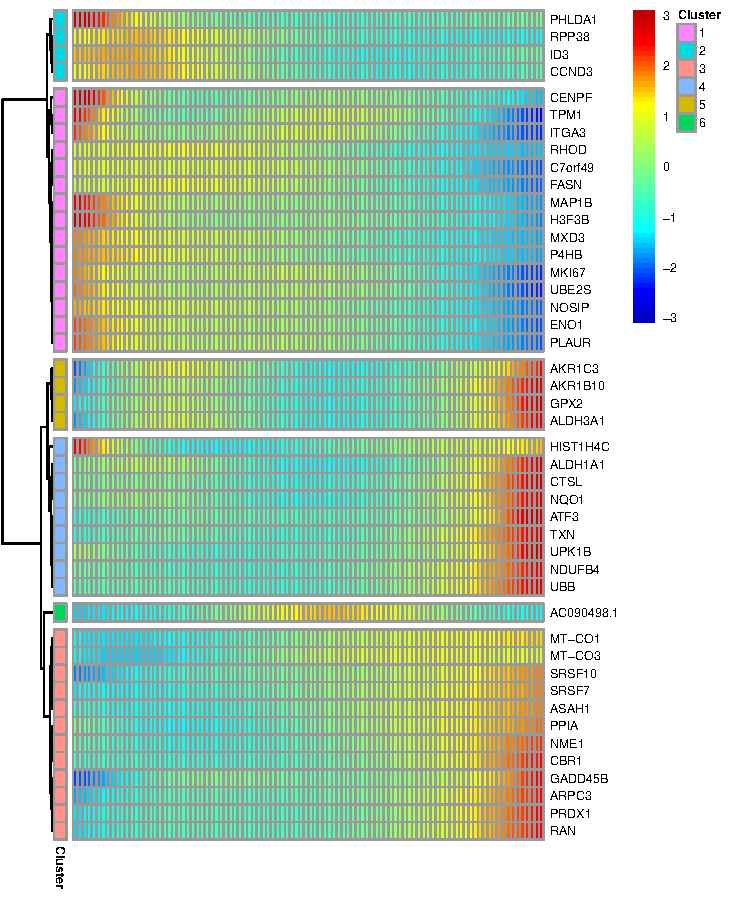
\includegraphics[width=0.7\linewidth]{figures/p_cellular_heatmap.pdf}}
\caption{\label{fig:cellulargenes}
Cellular genes that co-vary in expression along with the the amount of influenza virus mRNA in individual cells expressing all eight viral genes.
Shown are all genes that are differentially expressed at a false discovery rate of 0.1. 
Genes for which the color goes from blue at left to red at right are expressed at higher levels in cells with more viral mRNA. 
\jdbcomment{scale shows?} }
\figdata{The full results of the differential expression test is in \texttt{p\_sig\_cellular\_genes.csv}.}
\figdata{The results of a gene-set analysis are in \texttt{p\_sig\_cellular\_genes.csv}.}
\figsupp[Many genes that co-vary with the amount of viral mRNA are involved in the response to oxidative stress. \label{figsupp:ROStable}]{
Table delineating genes in (Figure~\ref{fig:cellulargenes}) that are associated with the response to oxidative stress ~\citep{Duong:2017ju,Jung:2017jz,Lee:2017ba,Peuchant:2017hj,MacLeod:2016kt,Jiang:2016cf,Gorrini:2013jv,Miura:2013fr,Kim:2009gi,Banning:2005cz,Murray:2003ie,Doyle:1999ts}.
}{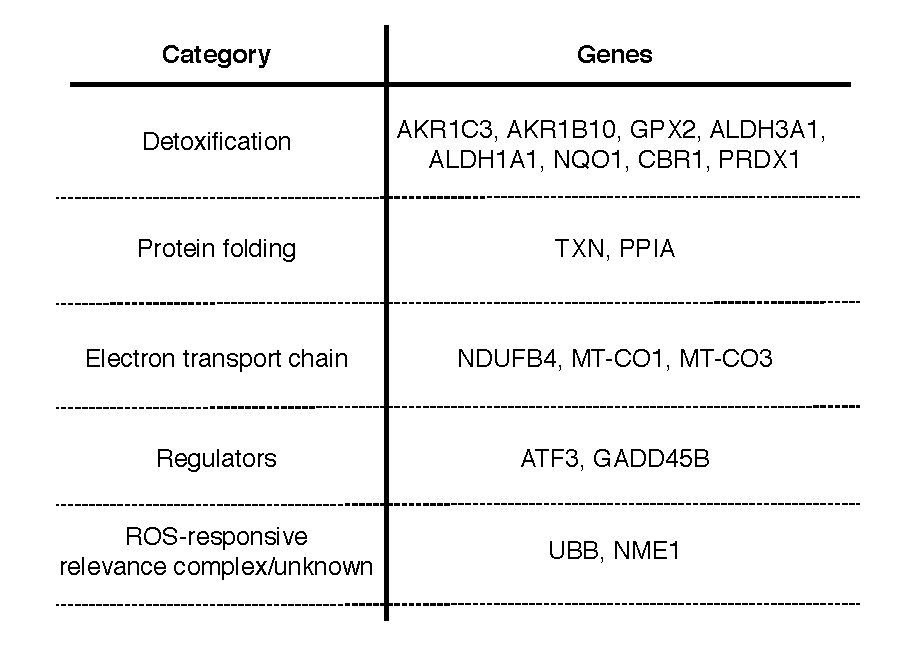
\includegraphics[width=0.7\linewidth]{figures/ROStable.pdf}}
\end{figure}

Many of the genes that exhibit increased expression in cells with large amounts of viral mRNA are known or suspected to be regulated by the Nrf2 master regulator in response to oxidative stress.
These genes produce proteins that are involved in detoxification of reactive oxygen species or resultant products, the management of misfolded proteins, the electron transport chain, or a general stress response (Figure~\ref{fig:cellulargenes}-Figure~supplement~\ref{figsupp:ROStable}). 
We additionally see reduced expression of the nitric oxide synthase interacting protein (NOSIP). 
Transient oxidative stress is known to occur during viral infection, and may act in a proviral fashion via MAPK activation driving vRNP export~\citep{Amatore:2014cs}.
The antioxidant response is thought to be largely antiviral, potentially through inhibition of MAPK activity \citep{Lin:2016ec,Sgarbanti:2014ht}.
Our data do not reveal whether the expression of genes involved in the response to oxidative stress are a cause or a symptom of higher levels of viral mRNA, and further investigation of this topic is an interesting area for future work.
Overall, the expression of some of the host genes in Figure~\ref{fig:cellulargenes}, along with inherent stochasticity and specific mutations to viral genes in individual cells, probably explain most of the variation in viral mRNA levels observed across the infected cells in our dataset.

\section{Discussion}
We have generated total transcriptome measurements of individual influenza-infected cells -- providing additional insight into the processes that drive influenza replication and its impact on the host at the cellular level.
Many of our observations closely match those made by other methods, validating our approach and granting us confidence in exploring more nuanced features of our data.
Overall we find that influenza replication is defined broadly by both significant stochasticity and significant robustness, and that a view of viral infection as either strictly deterministic or incredibly chaotic fails to accurately describe the infectious process.
Moreover we found that stress, likely induced by oxidative damage, appears to define the cellular response to infection.

One of the most striking features of stochasticity with respect to influenza infection is the absence of genes corresponding to a given genomic segment, observed both by ourselves and others~\citep{Brooke:2013kb,Dou:2017cp}
While there is significant speculation, and some indirect evidence, regarding the step of viral replication at which these genes are lost, there currently exists no strong consensus as to its identity -- indeed there may be no single event wholly responsible the stochastic loss of viral gene expression ~\citep{Brooke:2017gm, Heldt:2015iz}
Regardless it does not seem unreasonable to surmise that this is a consequence of possessing a segmented genome. If so, it can be reasonably concluded that at some phase of viral replication, whether packaging, delivery to the nucleus, production of replicative intermediates, or some as-yet unsurmised step, the components of the viral genome must act in at least a semi-independent fashion. 
A consequence of this stochasticity is a subpopulation of infected cells that express significantly lower levels of viral transcripts. 
Consistent with prior population-level studies of transcription, we find that absence of any of the four viral gene products necessary to form the viral polymerase leads to a dramatic drop in the levels of mRNA transcripts detected~\citep{Vreede:2004ip,eisfeld2015centre}. 
Our results are in slight contrast to a prior flow cytometric analysis of protein expression that described a relatively minor drop in expression associated with absence of viral ribonucleoprotein~\citep{Brooke:2013kb}.
This discrepancy could be explained by two possibilities. 
The first is that mRNA levels are not wholly predictive of viral protein abundance. 
The second is that flow cytometry depends on a user-defined dynamic range of sensitivity as well as positive and negative gates, and that the potential 2-3 log difference in population means was either not captured in the sensitivity of the instrument or that gates on positive populations excluded bone-fide positives. 
Indeed, gating on HA staining using a strict cutoff based on an uninfected population alone produces a curve that is consistent with a bimodal distribution of HA expression (Figure ~\ref{fig:coexpression} Figure Supplement ~\ref{figsupp:flowcyto}F).

However, despite extensive heterogeneity, there seems to be robustness to the infectious lifecycle.
For example, influenza, regardless of the viral burden, exhibits relatively constrained ratios between the viral transcripts.
This suggests that the processes that are driving heterogeneity of influenza mRNA abundance act equivalently throughout the viral genome.
Potential mechanisms include components such as binding and entry kinetics that act on a virion and thus on all segments packaged therein, limitations of transcription rate that are dependent upon the same pool of cellular resources, or potentially even feedback-dependent mechanisms controlling viral transcription. 

Perhaps even more important to influenza?s success in the face of stochasticity is the capacity of the virus to control the host innate immune response despite a large number of non-infectious events. 
While non-infectious events might be considered metabolic ?waste?, they would, theoretically, not impact the growth of successful viral infections. 
However, recognition of any virus, infectious or not, and production of interferon, would impact the entire viral population. 
While we cannot extrapolate much from our single interferon-positive cell, it can be stated that interferon induction by influenza is rare in our dataset. 
This is consistent with prior experiments using reporter cell lines,  which places the induction at ~1\% of cells with detectable influenza protein expression -- albeit this value is likely sensitive to differences in viral propagation and strain utilized ~\citep{Killip:2017ef, Chen:2010cr}. 
If the major influenza interferon antagonist, NS1, is absent in ~10-20\% of infections, and lowly expressed in those infections engaging in only primary transcription, we must posit that NS1 alone is insufficient to explain influenza evasion of innate immunity. 
Interestingly, if other segmented viruses also exhibit a pattern of stochastic segment loss, they too would need to overcome this hurdle and escape innate immunity through mechanisms relying on more than a gene product generated by a single segment.

In addition to viral mRNA kinetics, our analysis also allows us to observe those features of the cellular transcriptome that covary with influenza transcription.
Critically, our analysis does not require synchronization or infection with a high MOI, and thus avoids potential artifacts produced by either approach. 
We can therefore see extreme changes in a small subset of cells within a larger population.
Moreover, we can also observe how transcriptional changes partition between cells, and exclude dramatic changes such as interferon induction that, while important, can mask other interesting biologically-relevant responses. 
With this in mind, the predominant response associated with increased influenza mRNA transcript abundance appears to be the oxidative stress pathway. 
Generally characterized as antiviral, it is possible that cellular stress pathways represent an additional arm of innate immunity -- detecting a cellular state consistent with a loss of homeostasis as resources are diverted to viral propagation. 
Intriguingly, one element of the response, cyclophilin A (\emph{CypA}), is both thought to suppress influenza replication through degradation of matrix protein as well as act as a proinflammatory signal ~\citep{Liu:2009er, Jin:2004ii}.
It will be interesting to follow up on these observations and determine the broader mechanisms through which cellular stress pathways are involved in pro- or anti-viral responses.

The success garnered here underscores that single-cell approaches seem distinctly suited to study of viral pathogens, as not only are many host responses governed by bimodality and stochasticity ~\citep{Shalek:2014ey,Shalek:2013ej}, but also viral populations themselves exhibit a staggering array of diversity.
Our results with influenza have provided significant support for earlier analysis of viral stochasticity, further defined the sources and impacts of that stochasticity, and generated potentially fertile avenues of research. 
While it is early days yet, it is our hope that our efforts will contribute to a deeper understanding of viral populations, treating population-level measurements as emergent phenomena defined by underlying individual stochasticity rather than analyzing viral replication in a strictly deterministic framework.



\section{Methods and Materials}

\subsection{Cell lines and viruses}
The following cell lines were used in this study: the human lung epithelial carcinoma line A549 (ATCC CCL-185), the MDCK-SIAT1 variant of the Madin Darby canine kidney cell line overexpressing human SIAT1 (Sigma-Aldrich 05071502), and the human embryonic kidney cell line 293T (ATCC CRL-3216). 
All cells were maintained in D10 media (DMEM supplemented with 10\% heat-inactivated fetal bovine serum, 2 mM L-glutamine, 100 U of penicillin/ml, and 100 \si{\micro}g of streptomycin/ml) at 37 \si{\degreeCelsius} at 5 \% CO\textsubscript{2}.

Wildtype A/WSN/1933 (H1N1) influenza virus was generated by reverse genetics using the plasmids pHW181-PB2, pHW182-PB1, pHW183-PA, pHW184-HA, pHW185-NP, pHW186-NA, pHW187-M, and pHW188-NS~\citep{hoffmann2000dna}.
The sequences of the viral RNAs encoded in these plasmids are in Figure~\ref{fig:workflow}-source~data~\ref{figdata:viralsequences}.
Reverse-genetics plasmids encoding the synonymously barcoded WSN virus were created by using site-directed mutagenesis to introduce two synonymous mutations near the 3' end of the mRNA for each viral gene.
The synonymous mutations were chosen to introduce nucleotides that are common in naturally occurring H1N1 viruses to avoid unwanted attenuation.
The sequences of the synonymously barcoded viral RNAs are in Figure~\ref{fig:workflow}-source~data~\ref{figdata:viralsequences}
To generate viruses from these plasmids, we transfected an equimolar mix of all eight plasmids into cocultures of 293T and MDCK-SIAT1 cells seeded at a ratio of 8:1. 
At 24 hours post-transfection, we changed media from D10 to influenza growth media (Opti-MEM supplemented with 0.01\% heat-inactivated FBS, 0.3\% BSA, 100 U of penicillin/ml, 100  \si{\micro}g of streptomycin/ml, and 100 \si{\micro}g of calcium chloride/ml).
At 48 hours post-transfection we harvested the virus-containing supernatant, pelletted cellular material by centrifugation at 300 x g's for 4 minutes, and stored aliquots at of the clarified viral supernatant -80 \si{\degreeCelsius }. 
We then titered thawed aliquots of viral by TCID50 on MDCK-SIAT1 cells, computing titers via the formula of \citet{reed1938simple}.
To generate our ``high-purity'' stocks of viruses for the single-cell sequencing experiments, we then infected MDCK-SIAT1 cells at an MOI of 0.01, and let the virus replicate for 36 hours prior to harvesting aliquots that were again clarified by low-speed centrifugation, aliquoted, stored at -80  \si{\degreeCelsius }, and titered by TCID50.
The high-MOI passage (high-defective particle) stock used in Figure~\ref{fig:viruspopulations} was generated by instead passaging in MDCK-SIAT1 cells twice at an MOI of 1 for 48 hours, when obvious cytopathic effect was noted.

For the experiments in Figure~\ref{fig:coexpression}-Figure~supplement~\ref{figsupp:flowcyto}, we created a virus that carried an HA gene segment in which the carried GFP in place of most of the HA coding sequence by following a scheme first described by \citet{marsh2007specific}.
Briefly, we created a plasmid encoding a viral RNA with GFP in place of the HA coding sequence in the context of the pHH21~\citep{Neumann:1999ws} reverse-genetics plasmid, removing potential start codons upstream of the GFP (see Figure~\ref{fig:coexpression}-source~data~\ref{figdata:HAflank} for the sequence of the viral RNA)
We then generated GFP-carrying virus by reverse-genetics in previously described cells constitutively expressing HA~\citep{Doud:2016gm}.
A unidirectional vector for generating viral vRNA encoding eGFP flanked by HA packaging sequences was generated from a previously described vector, pHH21~\citep{Neumann:1999ws}. 
To obtain sufficient titers, this HA-eGFP virus was expanded for 44 than than 36 hours after initiating infection at an MOI of 0.01.

\subsection{qPCR}
For the qPCR in Figure~\ref{fig:viruspopulations} and Figure~\ref{fig:fluburdenbyflugene}-Figure~supplement~\ref{figsupp:cyclohexamide}, A549 cells were seeded at 3$\times$10\textsuperscript{5} cells / well in a 6-well tissue culture plate in D10 the day prior to infection. 
On the day of infection, a single well was trypsinized and the cells were counted in order to determine the appropriate amount of virus to use to achieve the intended MOI.
Immediately before infection, D10 was replaced with influenza growth media.
For cells incubated with cyclohexamide, the compound was added to a final concentration of 50  \si{\micro}g/ml at the time of infection -- previously confirmed to be sufficient to halt viral protein production~\citep{Killip:2014kz}.
RNA was purified using the QIAGEN RNeasy plus mini kit following manufacturer's instructions. 
cDNA was synthesized using an oligoDT primer and the SuperScript\textsuperscript{TM} III first-strand synthesis supermix from ThermoFisher using manufacturer's directions. 
Transcript abundance was measured using SYBR\textsuperscript{TM} green PCR master mix, using a combined anneal/extension step of 60 \si{\degreeCelsius } for one minute with the following primers: \emph{HA}: 5'-GGCCCAACCACACATTCAAC-3', 5'-GCTCATCACTGCTAGACGGG-3', \emph{IFNB1}: 5'-AAACTCATGAGCAGTCTGCA-3', 5'-AGGAGATCTTCAGTTTCGGAGG-3', \emph{L32}: 5'-AGCTCCCAAAAATAGACGCAC-3', 5'-TTCATAGCAGTAGGCACAAAGG-3'.   
Biological triplicates were performed for all samples.
For measurements of viral genomic HA content, vRNA was harvested from 80 \si{\micro}l of viral supernatant by the addition of 600 \si{\micro}l of RLT plus before proceeding with the standard QIAGEN Rneasy plus miniprep kit protocol, and cDNA was generated using  SuperScript\textsuperscript{TM} III first-strand synthesis supermix with primers specific for vRNA adapted from \citep{Hoffmann:2001vj}  using the manufacturer's protocol for random-hexamer priming~\citep{Xue:2017dl}.
qPCR was then performed as for mRNA measurements.
In order to obtain molecular resolution on our measurements of HA vRNA, a standard curve was generated from three independent dilutions of the HA-encoding reverse genetics plasmid. 
All vRNA values represent three independent RNA extractions with two replicate qPCR measurements. 

\subsection{Flow cytometry titering and analyses}
To determine viral titers in terms of HA-expressing units and for the flow cytometry in Figure~\ref{fig:coexpression}-Figure~supplement~\ref{figsupp:flowcyto}, A549 cells were seeded in a 6-well plate and infected as described above for the qPCR analyses.
Cells were harvested by trypsinization, resuspended in phosphate-buffered saline supplemented with 2\% heat-inactivated FBS, and stained with 10 \si{\micro}g/ml of H17-L19, a mouse monoclonal antibody confirmed to bind to WSN HA in a prior study~\citep{Doud:2017bw}.
After subsequent washes in supplemented PBS, cells were stained with a goat anti-mouse IgG antibody conjugated to APC.
Cells were then washed, fixed in 1\% formaldehyde, and washed further before a final resuspension and analysis. 
To determine HA-expressing units, we then determined the fraction of cells that were HA positive and calculated the HA-expressing units from these fractions assuming a Poisson infection process.

For Figure~\ref{fig:coexpression}-Figure~supplement~\ref{figsupp:flowcyto}, after gating to exclude multiplets in FlowJo, data were subsequently extracted using the R package flowCore~\citep{LeMeur:2007uo} and analyzed using a custom Python script.
Guassian kernel density estimates were obtained using the scipy stats package method, guassian\_kde, using automatic bandwidth determination~\citep{vanderWalt:2017dp}.

\subsection{Infections for single-cell mRNA sequencing}
Single cell sequencing libraries were generated using the 10x Chromium Single Cell 3' platform, V1~\cite{zheng2017massively}.
All time points except for the 8-hour repeat, were performed on the same day.

For the infections, A549 cells were seeded in a 6-well plate, with two wells per time point. 
A single well of cells was trypsinized and counted prior to initiation of the experiment for the purposes of calculating MOI.
Wild-type and synonymously barcoded virus were mixed to an estimated ratio of 1:1 based on prior, exploratory, single-cell analyses (data not shown). 
At the initiation of our experiment, the wells for all time points were changed from D10 to influenza growth media.
Cells were then infected with 0.3 HA-expressing units of virus per cell (a determined by flow cytometry).
The infections were performed in order of time point: first the 10-hour time point, then the 8-hour, and then the 6-hour time point.
At one hour after infection, the media for each time point was changed to fresh influenza growth media.
Note that the HA-expressing units were calculated without this additional washing step, and so likely represent an overestimate of our final infectious dose (consistent with the fact that fewer than 30\% of cells appear infected in the single-cell sequencing data).
All cells were then harvested for single-cell analysis concurrently -- ensuring all had spent equivalent time in changed media .
For our replicate 8-hour time point, cells were infected as above except that the cells were infected at 0.1 HA-expressing units of virus per cell but no wash step was performed, and the sample was prepared on a different day.
After harvest, cells were counted using disposable hemocytometers and diluted to equivalent concentrations with an intended capture of 3000 cells/sample following the manufacturer's provided by 10x Genomics for the Chromium Single Cell platform.
All subsequent steps through library preparation followed the manufacturer's protocol.
Samples were sequenced on an Illumina HiSeq. 
The deep sequencing data are available on the Sequence Read Archive under accession \jdbcomment{Jesse will upload and add this.}

\subsection{Computational analysis of single-cell mRNA sequencing data}
Jupyter notebooks that perform all of the computational analyses are available at \url{https://github.com/jbloomlab/flu_single_cell} \jdbcomment{This GitHub repository will be made public upon acceptance of the manuscript. If you are a reviewer who needs access, please contact the editor.}

Briefly, the raw deep sequencing data were processed using the 10X Genomics software package CellRanger (version 2.0.0).
The reads were aligned to a concatenation of the human and influenza virus transcriptomes.
The human transcriptome was generated by filtering genome assembly GRCh38 for protein coding genes defined in the GTF file GRCh38.87.
The influenza virus transcriptome was generated from the reverse-complement of the wildtype WSN viral RNA sequences as encoded in the reverse-genetics plasmids (Figure~\ref{fig:workflow}-source~data~\ref{figdata:viralsequences}).
CellRanger calls cells based on the number of observed cell barcodes, and creates a cell-gene matrix.
We used custom Python code to annotate the cells in this matrix by the number of viral reads that could be assigned to the wildtype and synonymously barcoded virus.
This annotated cell-gene matrix is in Supplementary~file~\ref{suppfile:cellgenematrix}.
The Jupyter notebook that performs these analyses is at \url{https://github.com/jbloomlab/flu_single_cell/blob/master/align_and_annotate.ipynb} \jdbcomment{This GitHub repository will be made public upon acceptance of the manuscript. If you are a reviewer who needs access, please contact the editor.}, and is also available as Supplementary~file~\ref{suppfile:alignandannotate}.

The annotated cell-gene matrix was then further analyzed in R, primarily using the Monocle package (version 2.4.0)~\citep{Qiu:2017dw,Trapnell:2014kg}.
The Jupyter notebook that performs these analyses is at \url{https://github.com/jbloomlab/flu_single_cell/blob/master/monocle_analysis.ipynb} \jdbcomment{This GitHub repository will be made public upon acceptance of the manuscript. If you are a reviewer who needs access, please contact the editor.}, and is also available as Supplementary~file~\ref{suppfile:monocle}.

Briefly, this analysis was performed as follows.
For each sample, cell barcodes with 2.5-fold fewer or more UMI counts mapping to cellular transcripts than the sample mean were considered to be potential doublets or inefficient/empty reactions, and were excluded from downstream analyses (see red vertical lines in Figure~\ref{fig:cells}C).
In order to determine an appropriate cutoff for how many reads a cell needed to contain in order to be classified as infected, we calculated the mean viral barcode purity across all cells that contained at least a given fraction of viral mRNA and had multiple viral reads that could be assigned a barcode (Figure~\ref{fig:viralbarcodes}B,C).
We then determined the threshold fraction of viral mRNA at which the mean purity no longer increased as a function of the amount of viral mRNA.
This threshold represents the point at which we have effectively eliminated cells that have low barcode purity simply due to lysis-acquired reads sampled randomly from both viral barcodes.
The 10-hour sample has the most viral mRNA, and is expected to have the most lysis-associated influenza reads.
We therefore determined the threshold using just this sample (Figure~\ref{fig:viralbarcodes}C), and then applied this threshold to all samples.
This procedure is expected to be conservative, and may miss some truly infected cells with very low amounts of viral mRNA.
For subsequent analyses, we retained all infected cells and a subsample of uninfected cells (the greater of 50 or the number of infected cells for that sample).
The rationale for subsampling the uninfected cell is that the vast majority of cells are uninfected, and we did not want these cells to completely dominate the t-SNE clustering and other downstream analyses.

For the semi-supervised t-SNE clustering, we used Monocle's cell hierarchy function to bin cells into those with no viral mRNA, <2\% viral mRNA, between 2\% and 20\% viral mRNA, and >20\%. 
Candidate marker genes t-SNE dimensionality reduction were then determined using the Monocle function markerDiffTable, excluding the effects of sample variation and the number of genes identified in a given cell, using a q-value cutoff of 0.01.
The specificity of these markers was determined using the function calculateMarkerSpecificity -- the top 40 markers were retained, and used to place populations in a two-dimensional plane based on tSNE dimensionality reduction.

For the analyses of cellular genes that differed in expression as a function of the amount of viral mRNA, we only considered cells that expressed all 8 viral mRNAs to avoid effects driven simply by viral gene absence.
We also only considered cellular genes in the differential gene analysis, since viral gene expression will tautologically co-vary with the amount of viral mRNA.
Additionally, because influenza virus has the capacity to degrade or prevent the synthesis of host mRNAs~\citep{BercovichKinori:2016iw} and contributes significantly to the total number UMIs in some cells, we calculate size factors (a scalar value representing efficiency of UMI capture) based on cellular transcripts alone. 
Finally, we assigned all cells a ceiling fraction of mRNA from virus of 25\% so that a few extremely high-expressing cells did not dominate. 
Cellular genes with expression that co-varied with the fraction of viral mRNAs in a cell were then determined using the Monocle differentialGeneTest, after removing variance explained by sample to sample variation. 
\label{fig:cellulargenes} shows all genes that were significantly associated with the fraction of mRNA from virus at a false discovery rate of 0.1.

\section{Acknowledgments}

Additional information can be given in the template, such as to not include funder information in the acknowledgments section.

\nocite{*} % This command displays all refs in the bib file
\bibliography{references}

\clearpage

\begin{suppfile}
\caption{\label{suppfile:cellgenematrix}
The annotated cell-gene matrix in Matrix Market Format.}
\end{suppfile}

\begin{suppfile}
\caption{\label{suppfile:alignandannotate}
Jupyter notebook that runs CellRanger to align and annotate the reads.
The ZIP file also includes associated custom scripts run by this notebook.}
\end{suppfile}

\begin{suppfile}
\caption{\label{suppfile:monocle}
Jupyter notebook that analyzes the cell-gene matrix, primarily using Monocle.}
\end{suppfile}

\end{document}


\end{document}